\chapter{Ionised Gas Distribution, Kinematics and Ionisation}
	\label{cha:gas}
The inter-stellar medium (ISM) in early-type galaxies (ETGs) has several components: a diffuse hot ($\sim 10^7 \, \mathrm{K}$) X-ray halo (with typical mass range $10^8$--$10^{10} \, \mathrm{M_\odot}$); warm ($\sim 10^4 \, \mathrm{K}$) ionised gas ($10^2$--$10^4 \, \mathrm{M_\odot}$), which can be more clumpy; and cold ($<10^2 \, \mathrm{K}$) atomic and molecular gas ($10^6$--$10^8 \, \mathrm{M_\odot}$), which generally confined to small (kpc or less) scale clouds. In this chapter we study the spatially resolved properties of the ionised gas component in radio galaxies (RGs) from the emission lines in the VIMOS and MUSE datacubes of the Southern Sample.

Using the methods described in Section \ref{subsec:EmissionFit} we find the best-fitting line-of-sight velocity distribution (LOSVD; assumed to be Gaussian in form and represented by the mean velocity and velocity dispersion only) for the ISM. As described in \ref{subsec:EmissionFit}, all emission lines are fitted with the same LOSVD, but with each individual line fitted with its own flux. In the cases of the [\ion{O}{iii}], [\ion{O{i}}] and [\ion{N}{ii}] doublets, the components of the doublets are fitted with a fixed flux ratio of 1:0.34; the [\ion{N}{i}] doublet has a ratio of 1:0.65 \citep{Safier1992}; and the components of the [\ion{O}{ii}] and [\ion{S}{ii}] doublets are fitted independently.

The chapter is structured as follows. First, the flux and equivalent width maps for each emission line within the relevant wavelength ranges of VIMOS and MUSE are shown. Gas masses are calculated and upper limits given in the cases of non-detections (see Section \ref{sec:GasFlux}). Secondly, in Section \ref{sec:GasKin}, the kinematics of the ionised gas is discussed. Thirdly, the source of the ionising potential is investigated, making use of several emission line diagnostics (see Section \ref{sec:Diagnostics}). Finally we finish in Section \ref{sec:discuss} with a discussion of the results of this chapter.


\section{Ionised Gas Fluxes}
	\label{sec:GasFlux}
	\subsection{Maps}
		\label{subsec:GasMaps}
		Images of each galaxy in the Southern Sample in [\ion{O}{iii}]$\lambda\lambda$4957,5007 is shown in Figs.\ref{fig:VIMOS_OIII} and \ref{fig:MUSE_OIII}. Only 4 galaxies of the Southern Sample have detections of emission lines outside of the central region (IC 1459, NGC 612, NGC 1316 and NGC 3100; see Figs.\,\ref{fig:VIMOS_OIII} and \ref{fig:MUSE_OIII}). Of the remaining 7 galaxies, NGC 1399 and PKS 718-34 have no detection of H$\beta$ in the spatially resolved maps (we do find a detection in the spatially integrated spectrum of NGC 1399; see Section \ref{subsec:GasMass}), while the remaining 5 galaxies have detections only in the centre. All other emission lines have similar distribution, but at different intensities.%, with the exception of NGC 612, where the significant cloud in [\ion{O}{iii}] to the south of the centre of the galaxy is not seen in H\,$\beta$ (see Fig.\,\ref{fig:NGC612_Hb}). 


		\begin{figure}
			\centering
			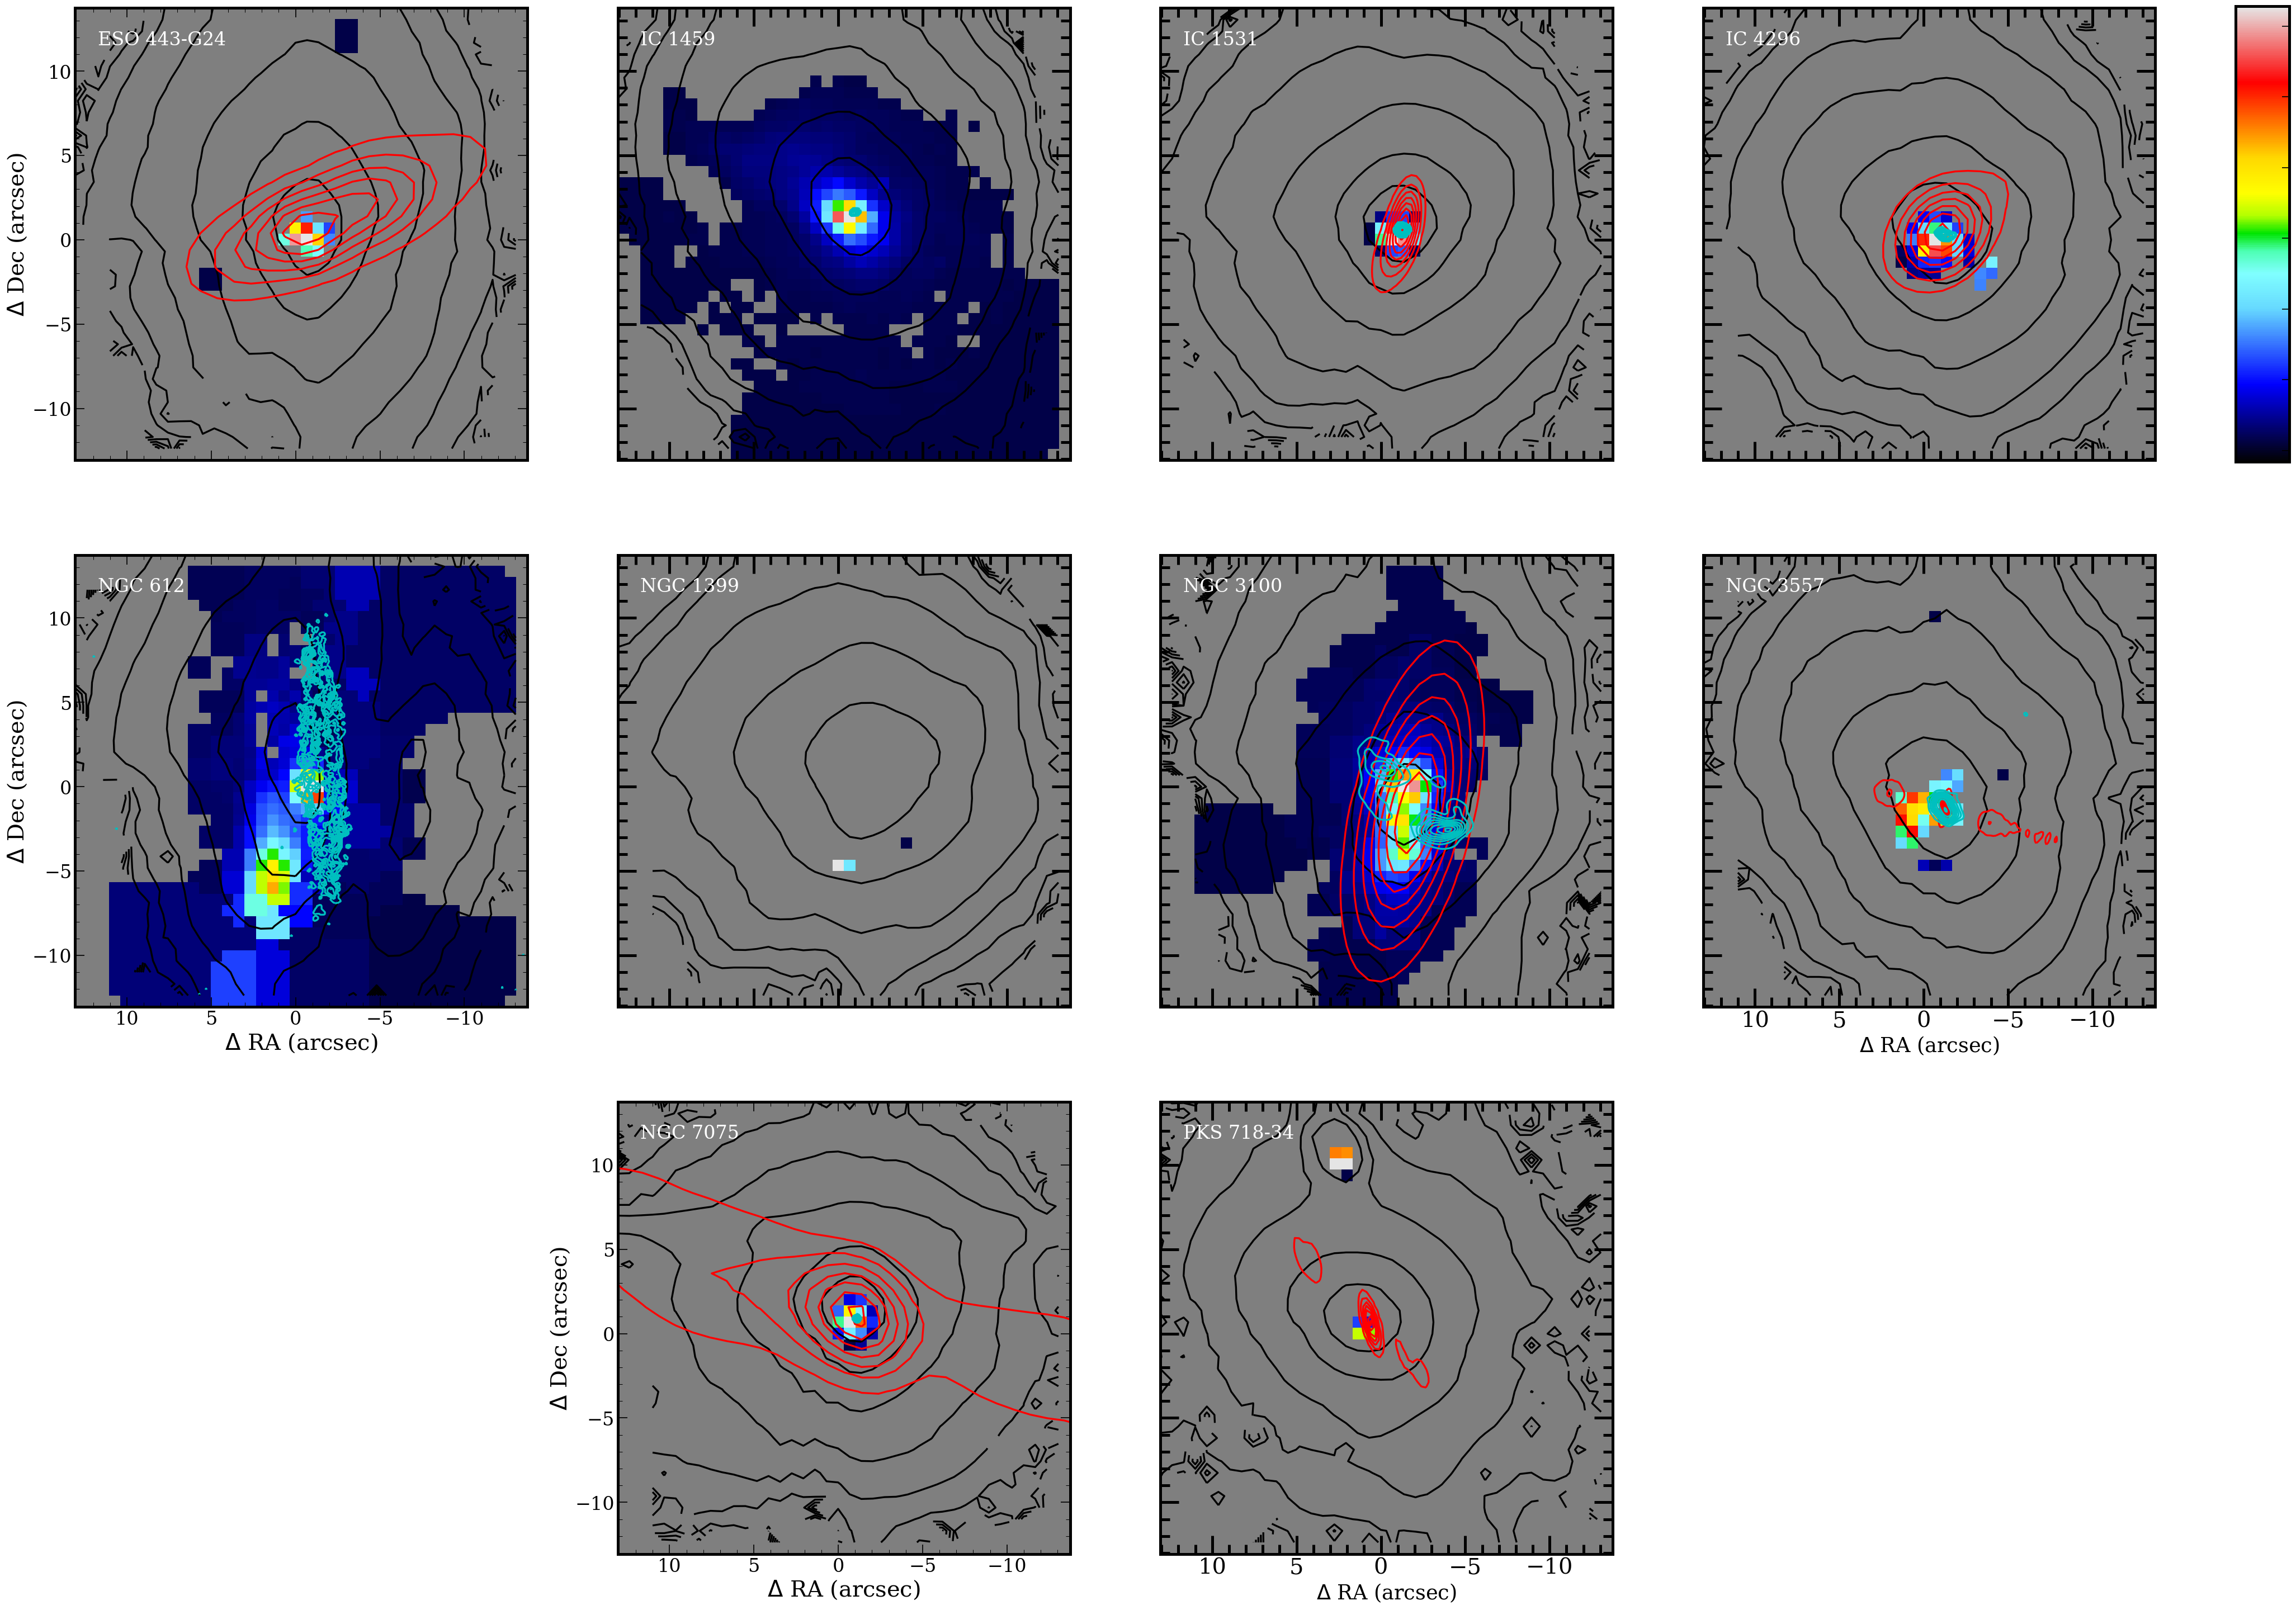
\includegraphics[width=\textwidth]{chapter5/vimos/Hb.png}
			\caption[VIMOS \bracket{\ion{O}{iii}} maps]{VIMOS [\ion{O}{iii}]$\lambda\lambda$4957,5007 maps.} 
			\label{fig:VIMOS_OIII}
		\end{figure}
		\begin{figure}
			\centering
			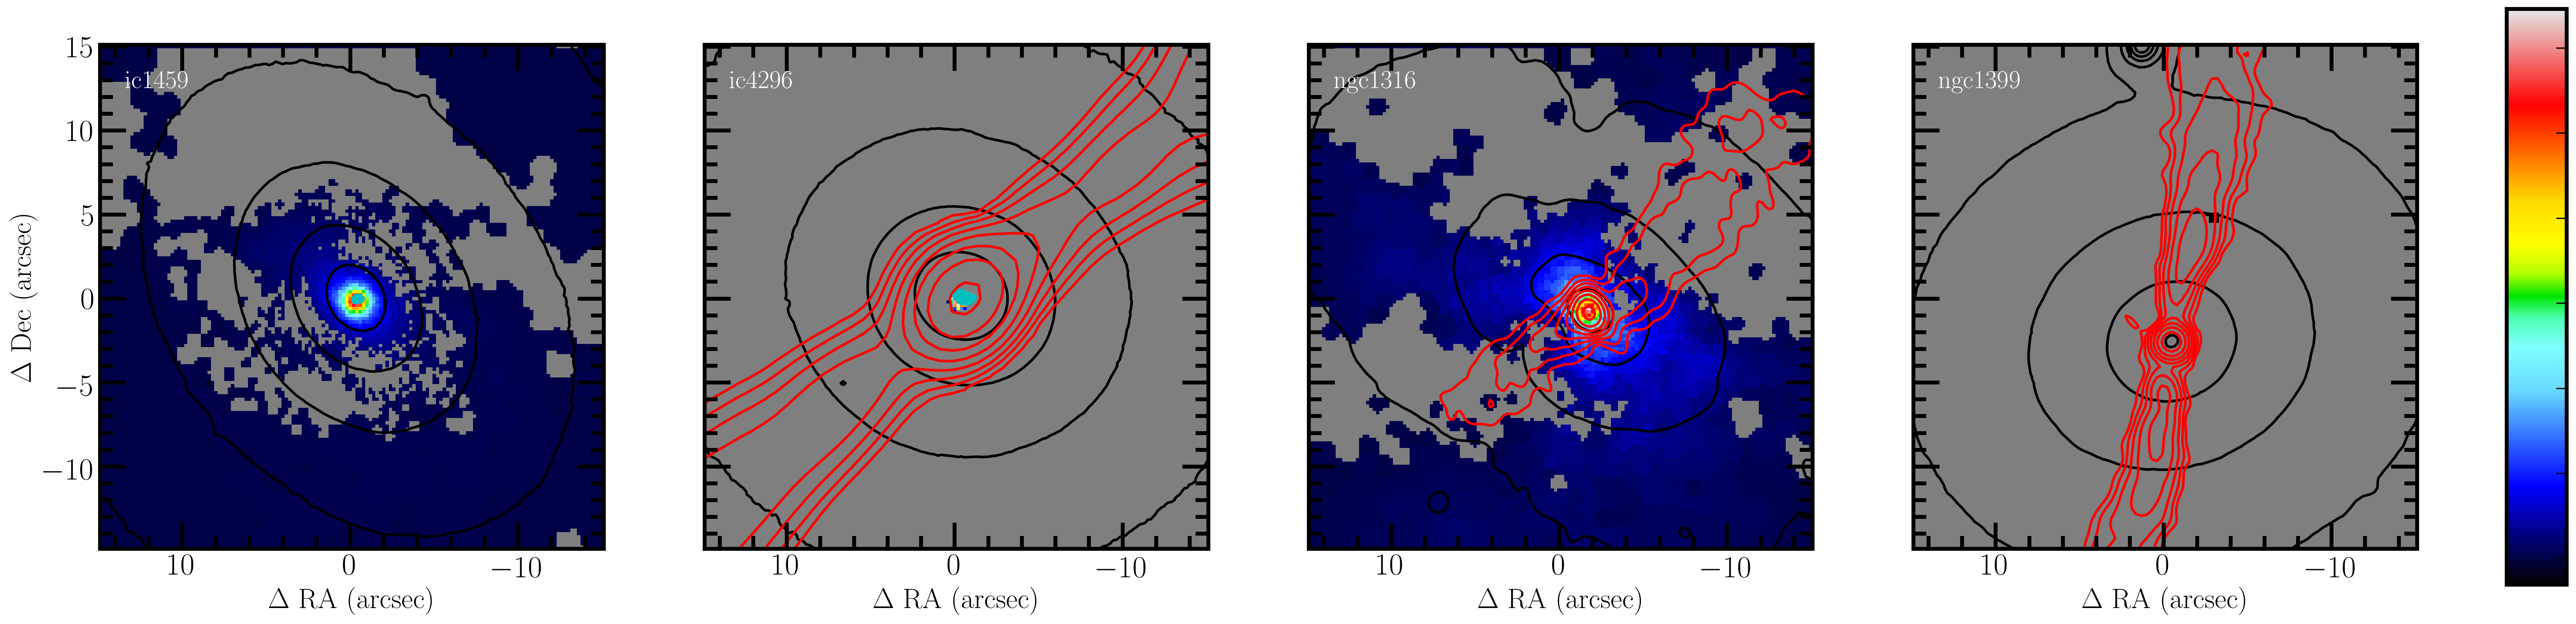
\includegraphics[width=\textwidth]{chapter5/muse/Hb.png}
			\caption[MUSE \bracket{\ion{O}{iii}} maps]{MUSE [\ion{O}{iii}]$\lambda\lambda$4957,5007 maps.} 
			\label{fig:MUSE_OIII}
		\end{figure}


		% \begin{figure}
		% 	\centering
		% 	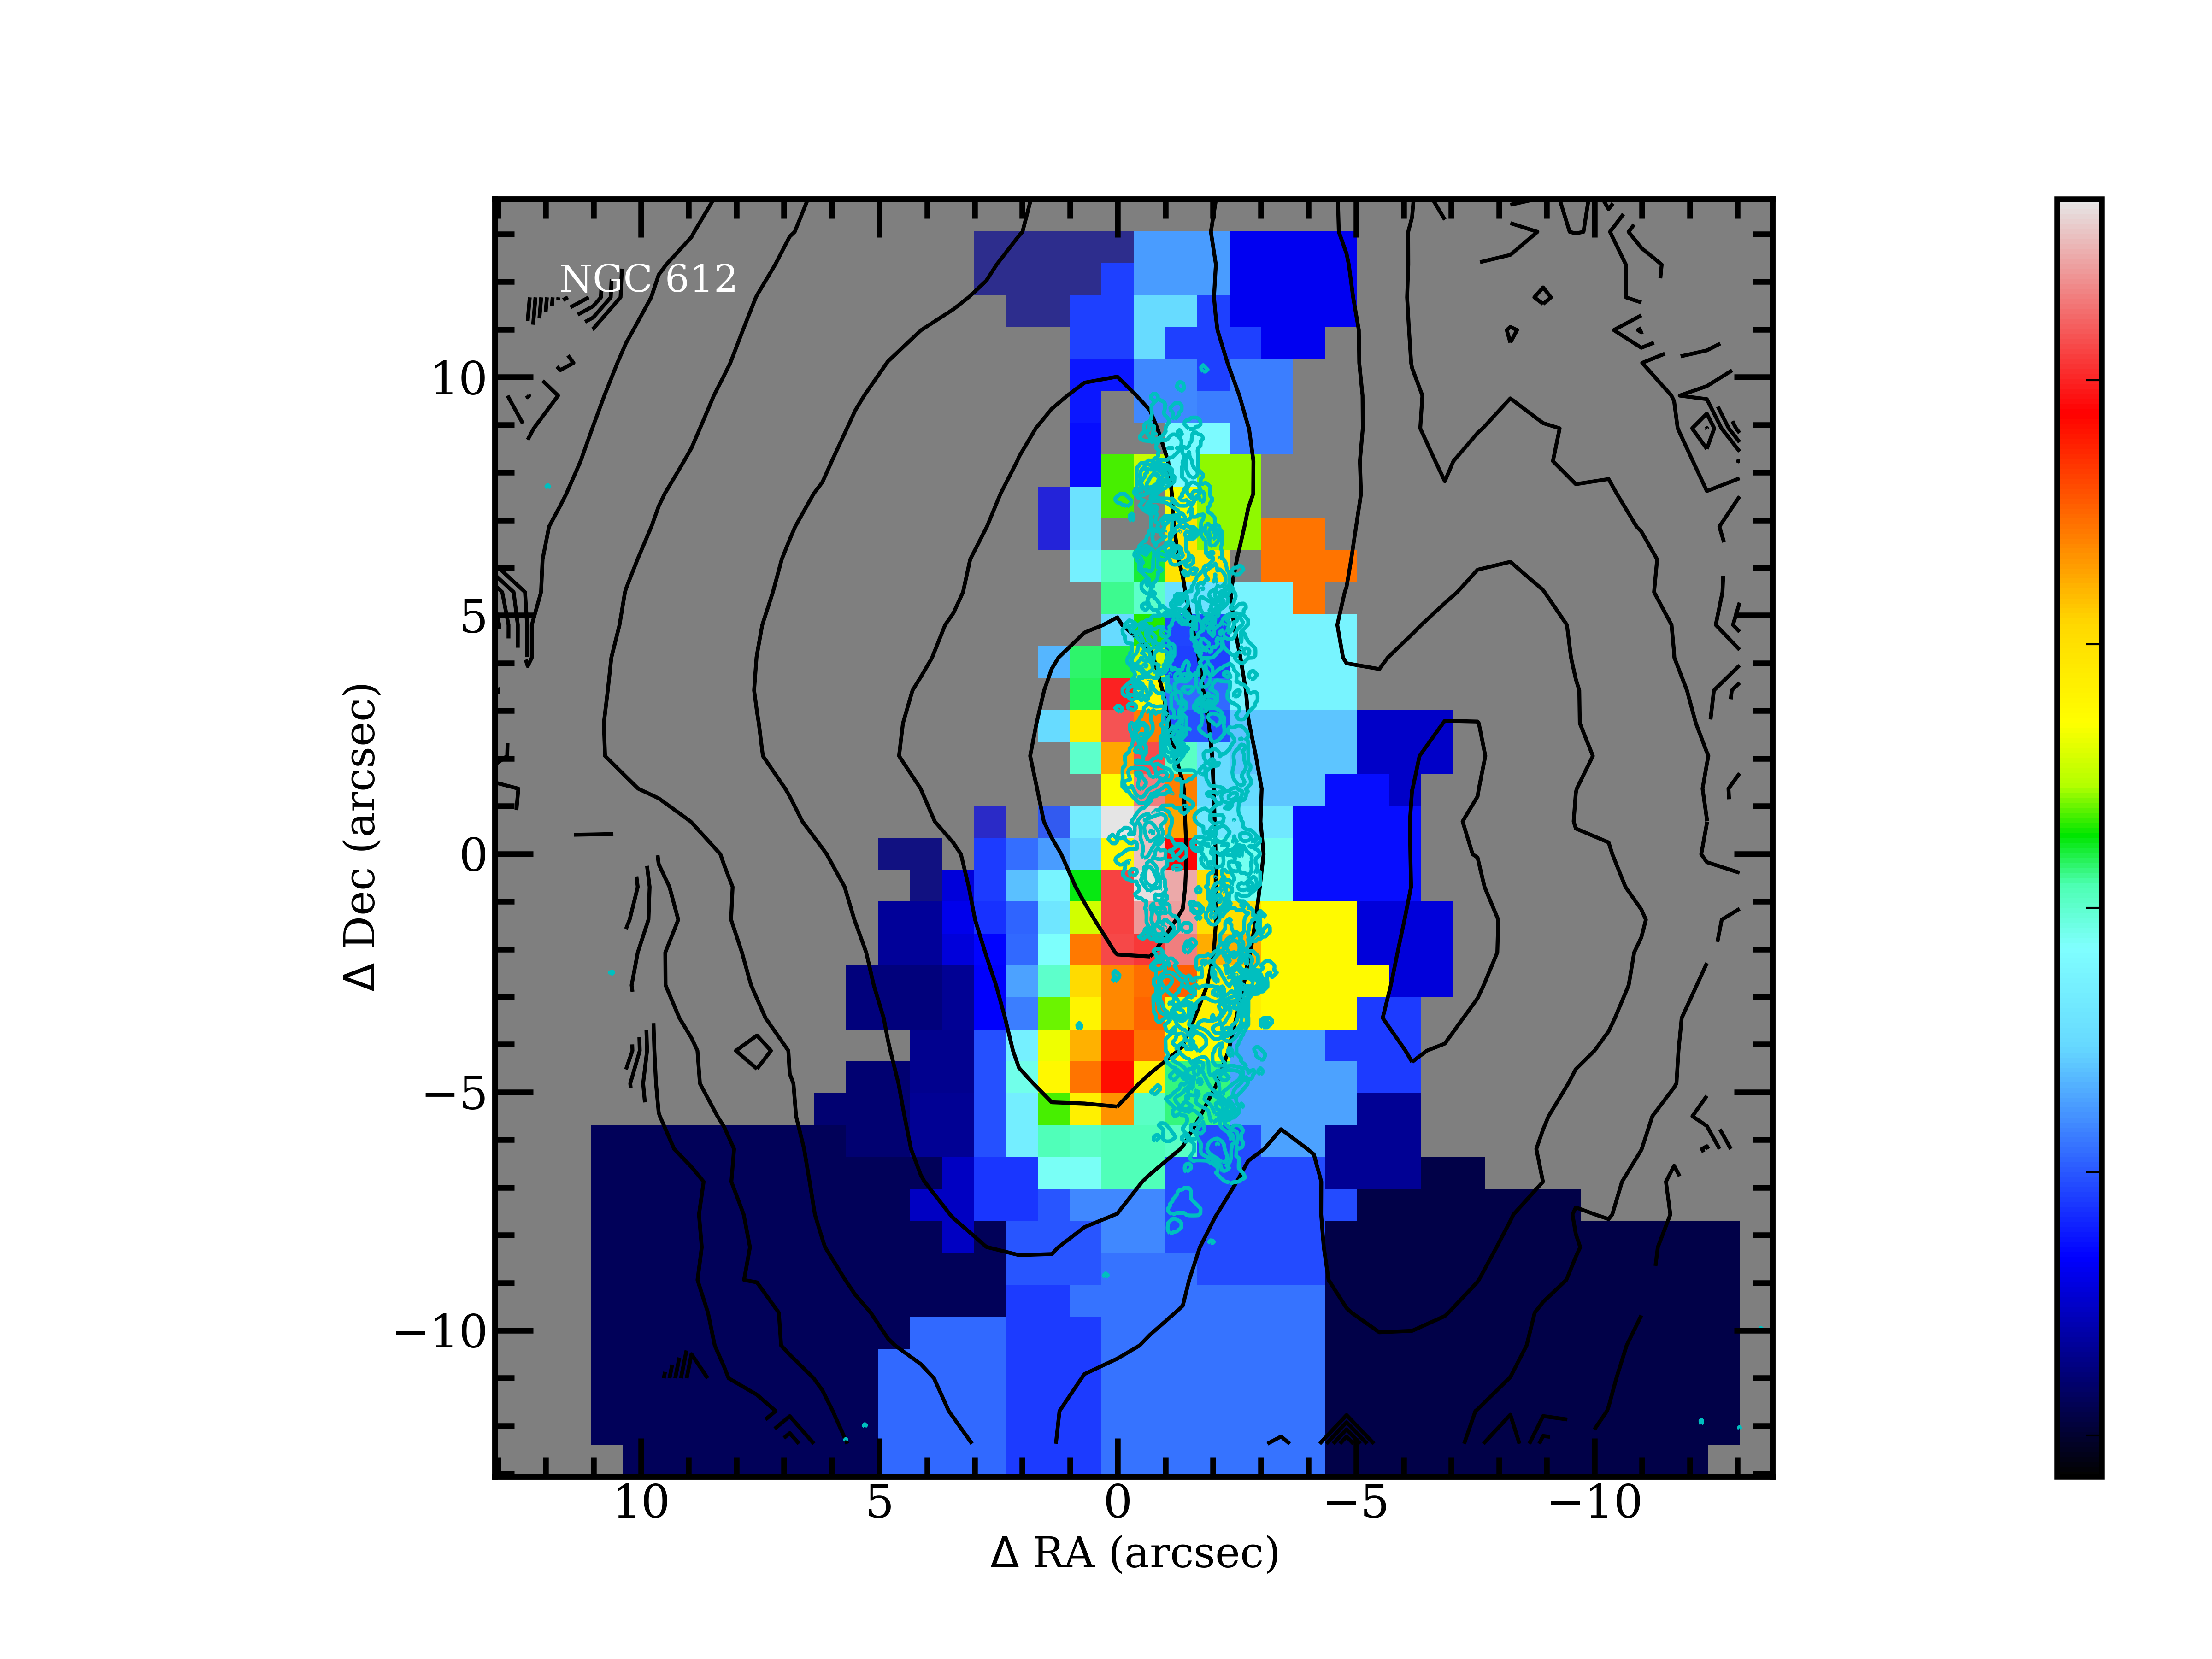
\includegraphics[width=0.4\textwidth]{chapter5/vimos/ngc0612_Hb.png}
		% 	\caption[NGC 612 H\,$\beta$ image]{NGC 612 H\,$\beta$ map showing a large cloud to the south of the centre of the galaxy, which is not present in the H$\beta$ map (see Fig.\ref{fig:VIMOS_Hb}).} 
		% 	\label{fig:NGC612_Hb}
		% \end{figure}


		% Because equivalent width is not dependent on overall intensity (except for the initial detection threshold: a line must be detected in order to observe its equivalent width), it can be used to highlight local structures that cannot be seen in flux maps. The equivalent width maps for each emission line for each galaxy in the Southern Sample are shown in Figs.\,\ref{fig:VIMOS_ew} and \ref{fig:MUSE_ew}. 

		% \begin{figure}
		% 	\centering
		% 	\includegraphics[width=\textwidth]{chapter5/vimos/ew.png}
		% 	\caption[VIMOS equivalent width maps]{VIMOS equivalent width maps.} 
		% 	\label{fig:VIMOS_ew}
		% \end{figure}
		% \begin{figure}
		% 	\centering
		% 	\includegraphics[width=\textwidth]{chapter5/muse/ew.png}
		% 	\caption[MUSE equivalent width maps]{MUSE equivalent width maps.} 
		% 	\label{fig:MUSE_ew}
		% \end{figure}

	\subsection{Gas Masses}
		\label{subsec:GasMass}

		Gas masses are derived using the recipe from \citet{Sarzi2005}. This is very rough calculation and the values should not be used for quantitative applications. The approach follows \citet{Kim1989}, and as such
		\begin{equation}
			M_\text{\ion{H}{ii}} = 280 \left(\frac{D}{10\, \mathrm{Mpc}}\right)^2 \frac{F(\mathrm{H\alpha})}{10^{-14} \, \mathrm{erg \, s^{-1} \, cm^{-2}}} \frac{10^3 \, \mathrm{cm^{-3}}}{n_\mathrm{e}} \, ,
		\end{equation}
		where $M_\text{\ion{H}{ii}}$ is the mass in solar mass ($M_\odot$) of \ion{H}{ii} in a galaxy $D$ Mpc away, with an observed H\,$\alpha$ flux of $F(\mathrm{H\,\alpha})$. This method assumes an electron density of $n_\mathrm{e} = 100 \, \mathrm{cm^{-3}}$, a temperature of $10^4$ K and case-B recombinations (electrons above 13.6\,eV are not reabsorbed; \citealt[e.g.][p.\,74]{Osterbrock1974}). Like \citet{Sarzi2005}, we only claim a detection if the amplitude-to-noise ratio (A/N) is $>4$ for [\ion{O}{iii}] and $>2.5$ for H\,$\beta$ or H\,$\alpha$. Since most of the gas is centrally concentrated using a large field of view, often only serves to increase the noise (reducing A/N). 
		% Our lower limits on the gas mass, are set by the mass measured from the largest aperture that still meets our detection criteria. This would be the gas mass of the galaxy if there was no gas at larger radii. 
		Upper limits are set by the mass found from the residual noise level (see Section \ref{subsec:EmissionFit}) or the H\,$\alpha$ (H\,$\beta$, in the case of VIMOS data) flux measurement which does not meet out A/N criteria, whichever is larger, for the entire field of view.


		\begin{table}
			\centering
		\begin{threeparttable}
			\caption{Gas Masses for the Southern Sample.}
			\label{tab:gasMass}
			% \begin{tabular*}{\textwidth}{@{\extracolsep{\fill}}l r r r l}
			\begin{tabular}{l c c c c}
				\hline
				\hline
				Galaxy & \multicolumn{2}{c}{\ion{H}{ii} Mass} & Balmer & LINER/ \\
				& VIMOS\tnote{a} & MUSE & Decrement & Seyfert \\
				& ($\log\mathrm{M_\odot}$) & ($\log\mathrm{M_\odot}$) & \\
				\hline
				ESO 443-G024 & $2.19 \pm 0.01$ 	& --  		& -- & -- \\
				IC 1459 	& $2.14 \pm 0.01$	& $1.24 \pm 0.01$ & $4.57 \pm 0.06$ & LINER-AGN\\
				IC 1531 	& $2.25 \pm 0.01$	& -- 		& -- & Seyfert 2\\
				IC 4296		& $2.31 \pm 0.01$	& $0.81 \pm 0.01$ & \tnote{b} & LINER-AGN \\
				NGC 612 	& $3.10 \pm 0.01$ 	& -- 		& -- & LINER-AGN \\
				NGC 1316 	& -- 				& $ 1.03 \pm 0.01$ & $3.54 \pm 0.05$ & LINER-AGN \\
				NGC 1399 	& $1.22 \pm 0.01$ 	& $ 0.29 \pm 0.01$ & \tnote{b} & LINER \\
				NGC 3100 	& $2.17 \pm 0.01$	& -- 		& -- & Seyfert 2 \\
				NGC 3557 	& $1.77 \pm 0.01$ 	& -- 		& -- & LINER/Retired \\
				NGC 7075 	& $2.40 \pm 0.01$	& -- 		& -- & LINER \\
				PKS 718-34  & --		 		& -- 		& -- & -- \\
				\hline
				\hline
			\end{tabular}
			\begin{tablenotes}
			\footnotesize
			\note Col.\,1: Galaxy. Col.\,2: \ion{H}{ii} mass derived from the H\,$\beta$ line in the VIMOS data, assuming a Balmer decrement of 2.85. Col.\,3: \ion{H}{ii} mass derived from the H\,$\alpha$ line in the MUSE data. Col.\,4: Observed Balmer decrement derived from the MUSE data. Col.\,5: Main source of ionizing radiation (see Section \ref{sec:Diagnostics} for a description of classification methods.)
			\item [a] VIMOS flux calibration is only approximate and these values to should be taken as such (see Section \ref{subsec:VIMOSreduction} for more detail about the flux calibration methods.)
			\item [b] H$\beta$ was not detected in either IC 4296 or NGC 1399, thus the formal observed Balmer decrement is $\infty$.

			% \item [b] H$\beta$ was not detected with an A/N $> 2.5$ meaning that the fit is not reliable (hence this is an upper limit). 
			\end{tablenotes}
		\end{threeparttable}
		\end{table}
		

% So what?




\section{Ionised Gas Kinematics}
	\label{sec:GasKin}
	In Figs.\,\ref{fig:VIMOS_Gaskine} and \ref{fig:MUSE_Gaskine}, we show the maps of the mean velocity and velocity dispersion for the ISM in the galaxies with a significant number of spatial bins that have gas detected in our Southern sample (IC 1459, NGC 612, NGC 1316 and NGC 3100). Due to that fact that, unlike stars, gas is not frictionless, with a long enough period of time after an interaction the ISM will always settle into a disc. These maps show that the Southern sample vary from very settled discs in IC 1459 and NGC 612, to more disordered kinematics and a possible inflow in NGC 1316.

	\begin{figure}
		\centering
		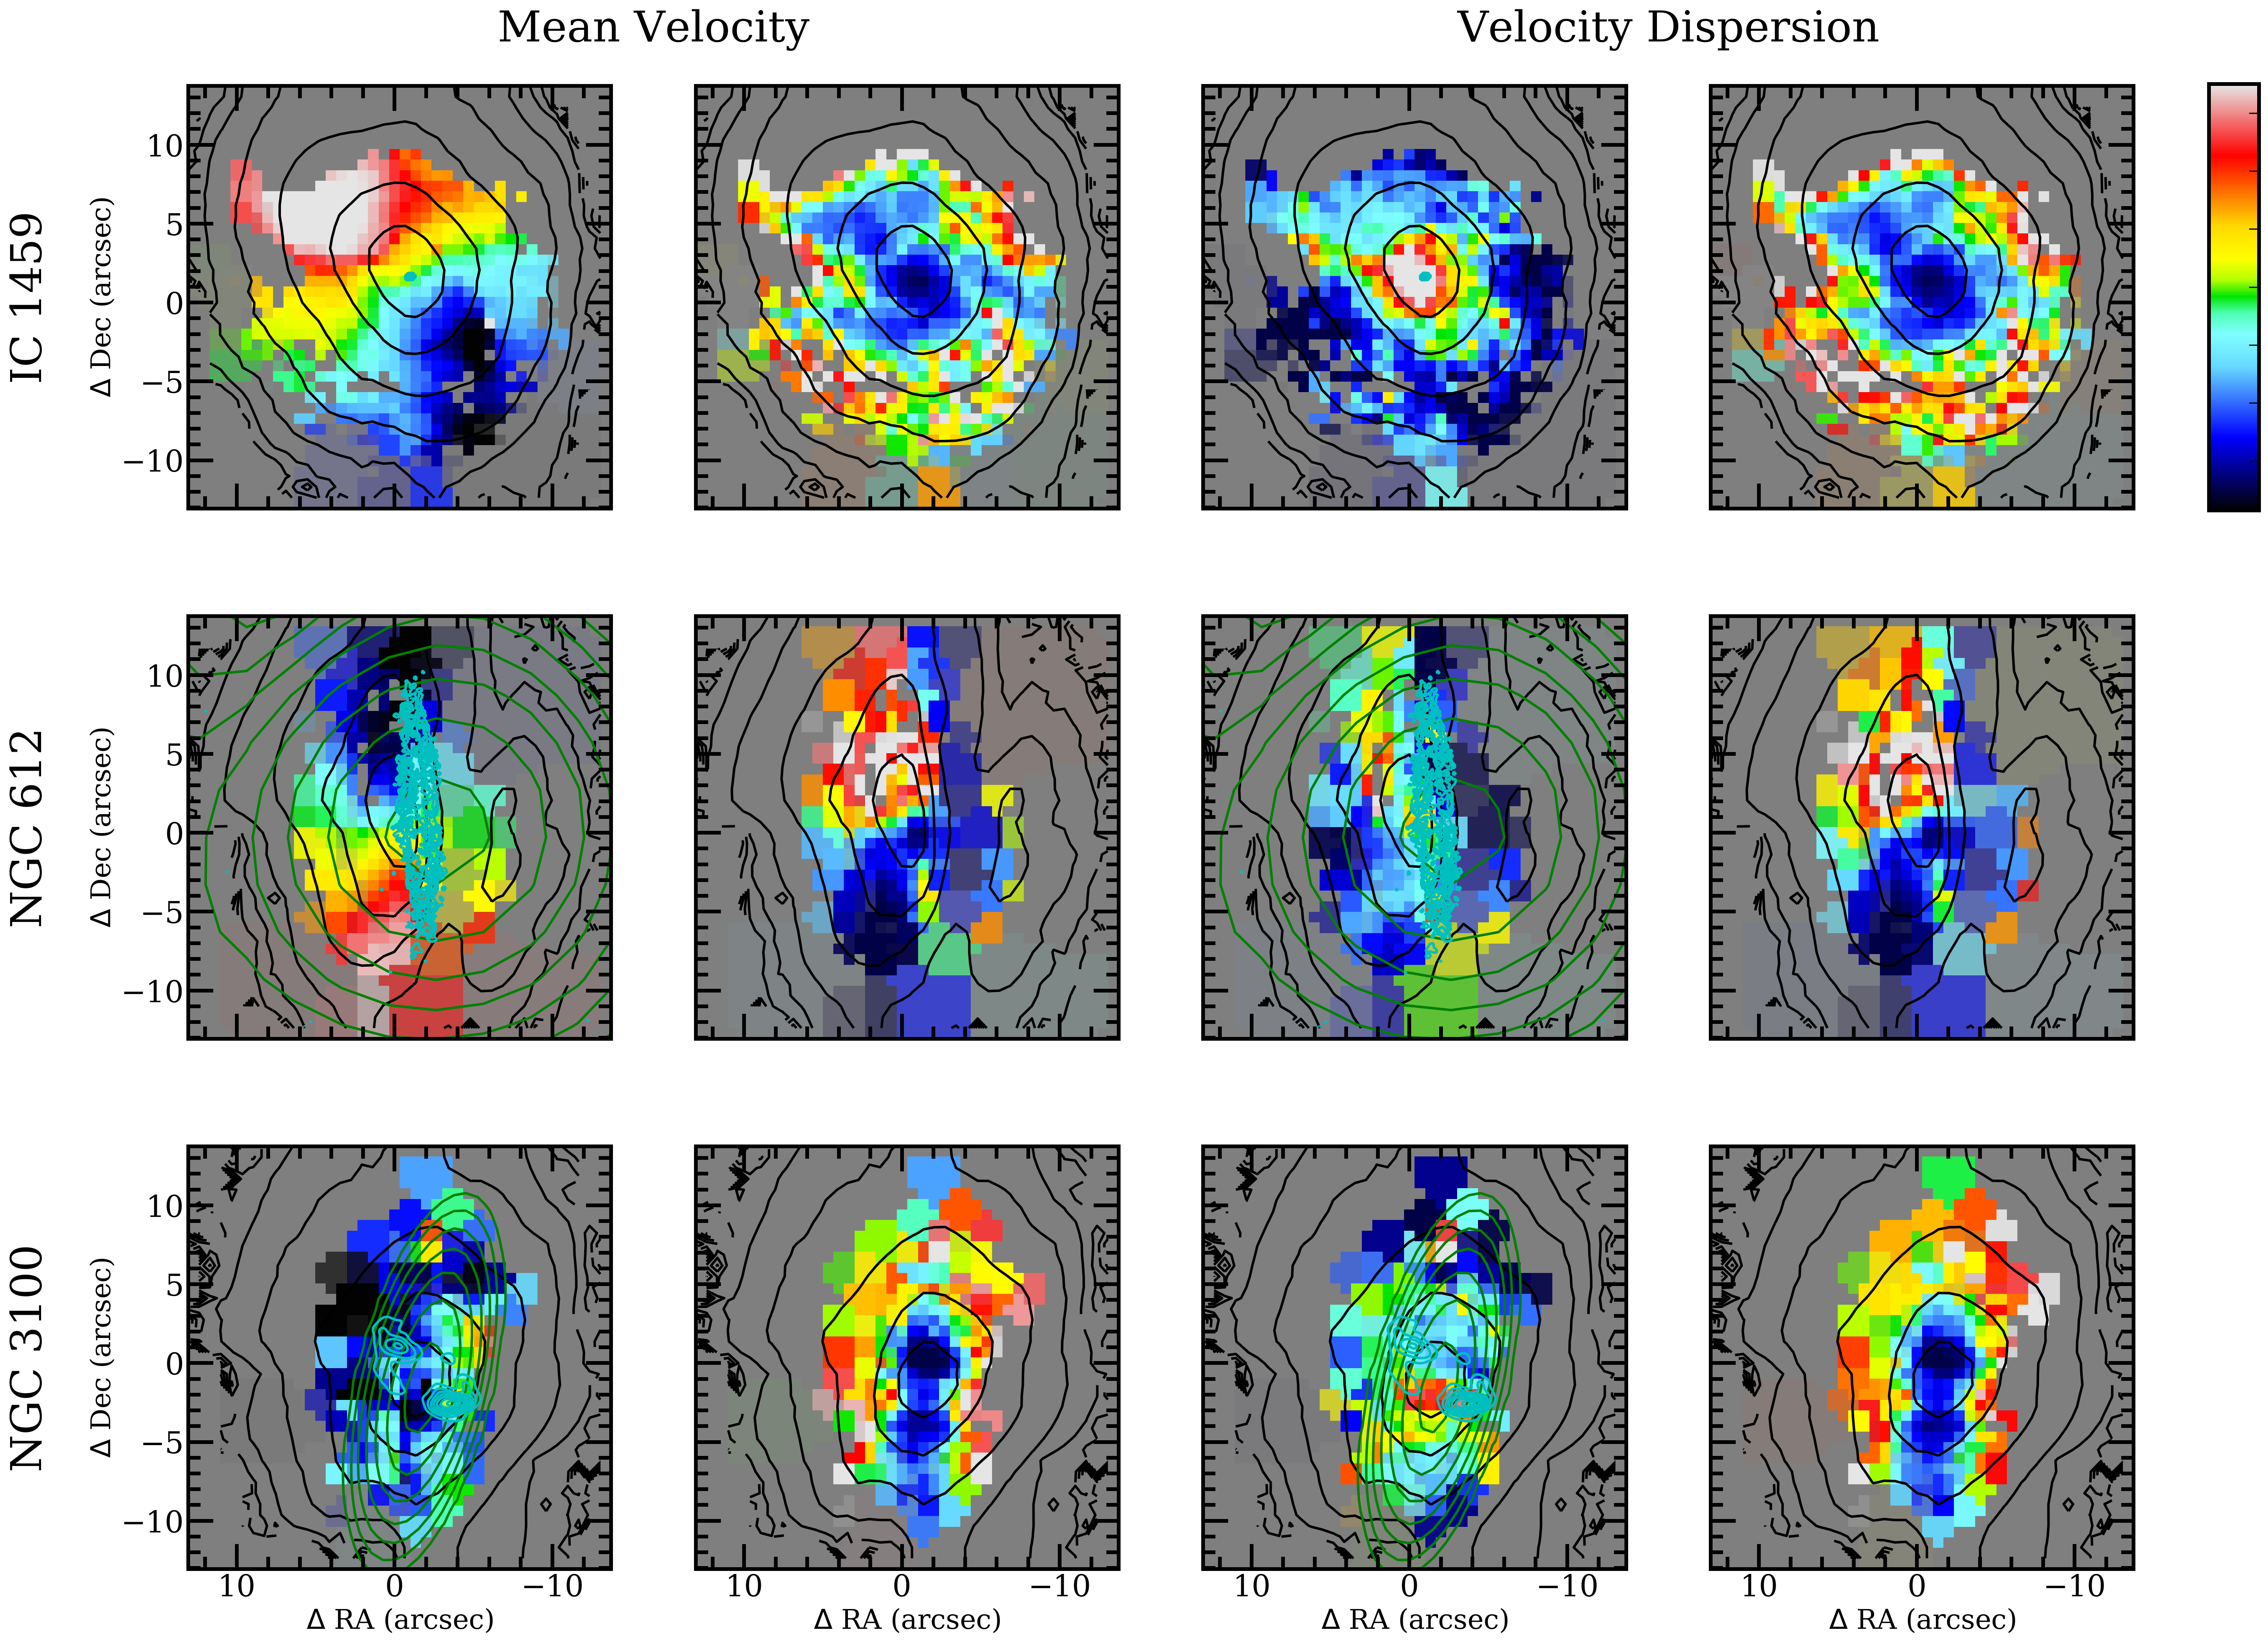
\includegraphics[height=0.47\textheight]{chapter5/vimos/kin.png}
		\caption[VIMOS ISM kinematic maps]{VIMOS ISM kinematic maps. Left to right: mean velocity and velocity dispersion. Alternate columns show a given parameter its associated uncertainty. Top to bottom: IC 1459, NGC 612 and NGC 3100. Flux contours (isophotes) are shown in black, \ce{^{12}CO(2-1)} contours from ALMA in cyan and radio continuum contours from VLA in green. The radio band displayed depends on the data available in the archive and which images had a similar resolution and scales. Limits on the colour scale are: mean velocity maps -360 to 360\,$\mathrm{km \, s^{-1}}$ (except for NGC 3100 which has limits of -100 to 100\,$\mathrm{km \, s^{-1}}$), mean velocity uncertainty 1 to 15\,$\mathrm{km \, s^{-1}}$, velocity dispersion 35 to 200\,$\mathrm{km \, s^{-1}}$ and velocity dispersion uncertainty 1 to 20\,$\mathrm{km \, s^{-1}}$.} 
		\label{fig:VIMOS_Gaskine}
	\end{figure}

	\begin{figure}
		\centering
		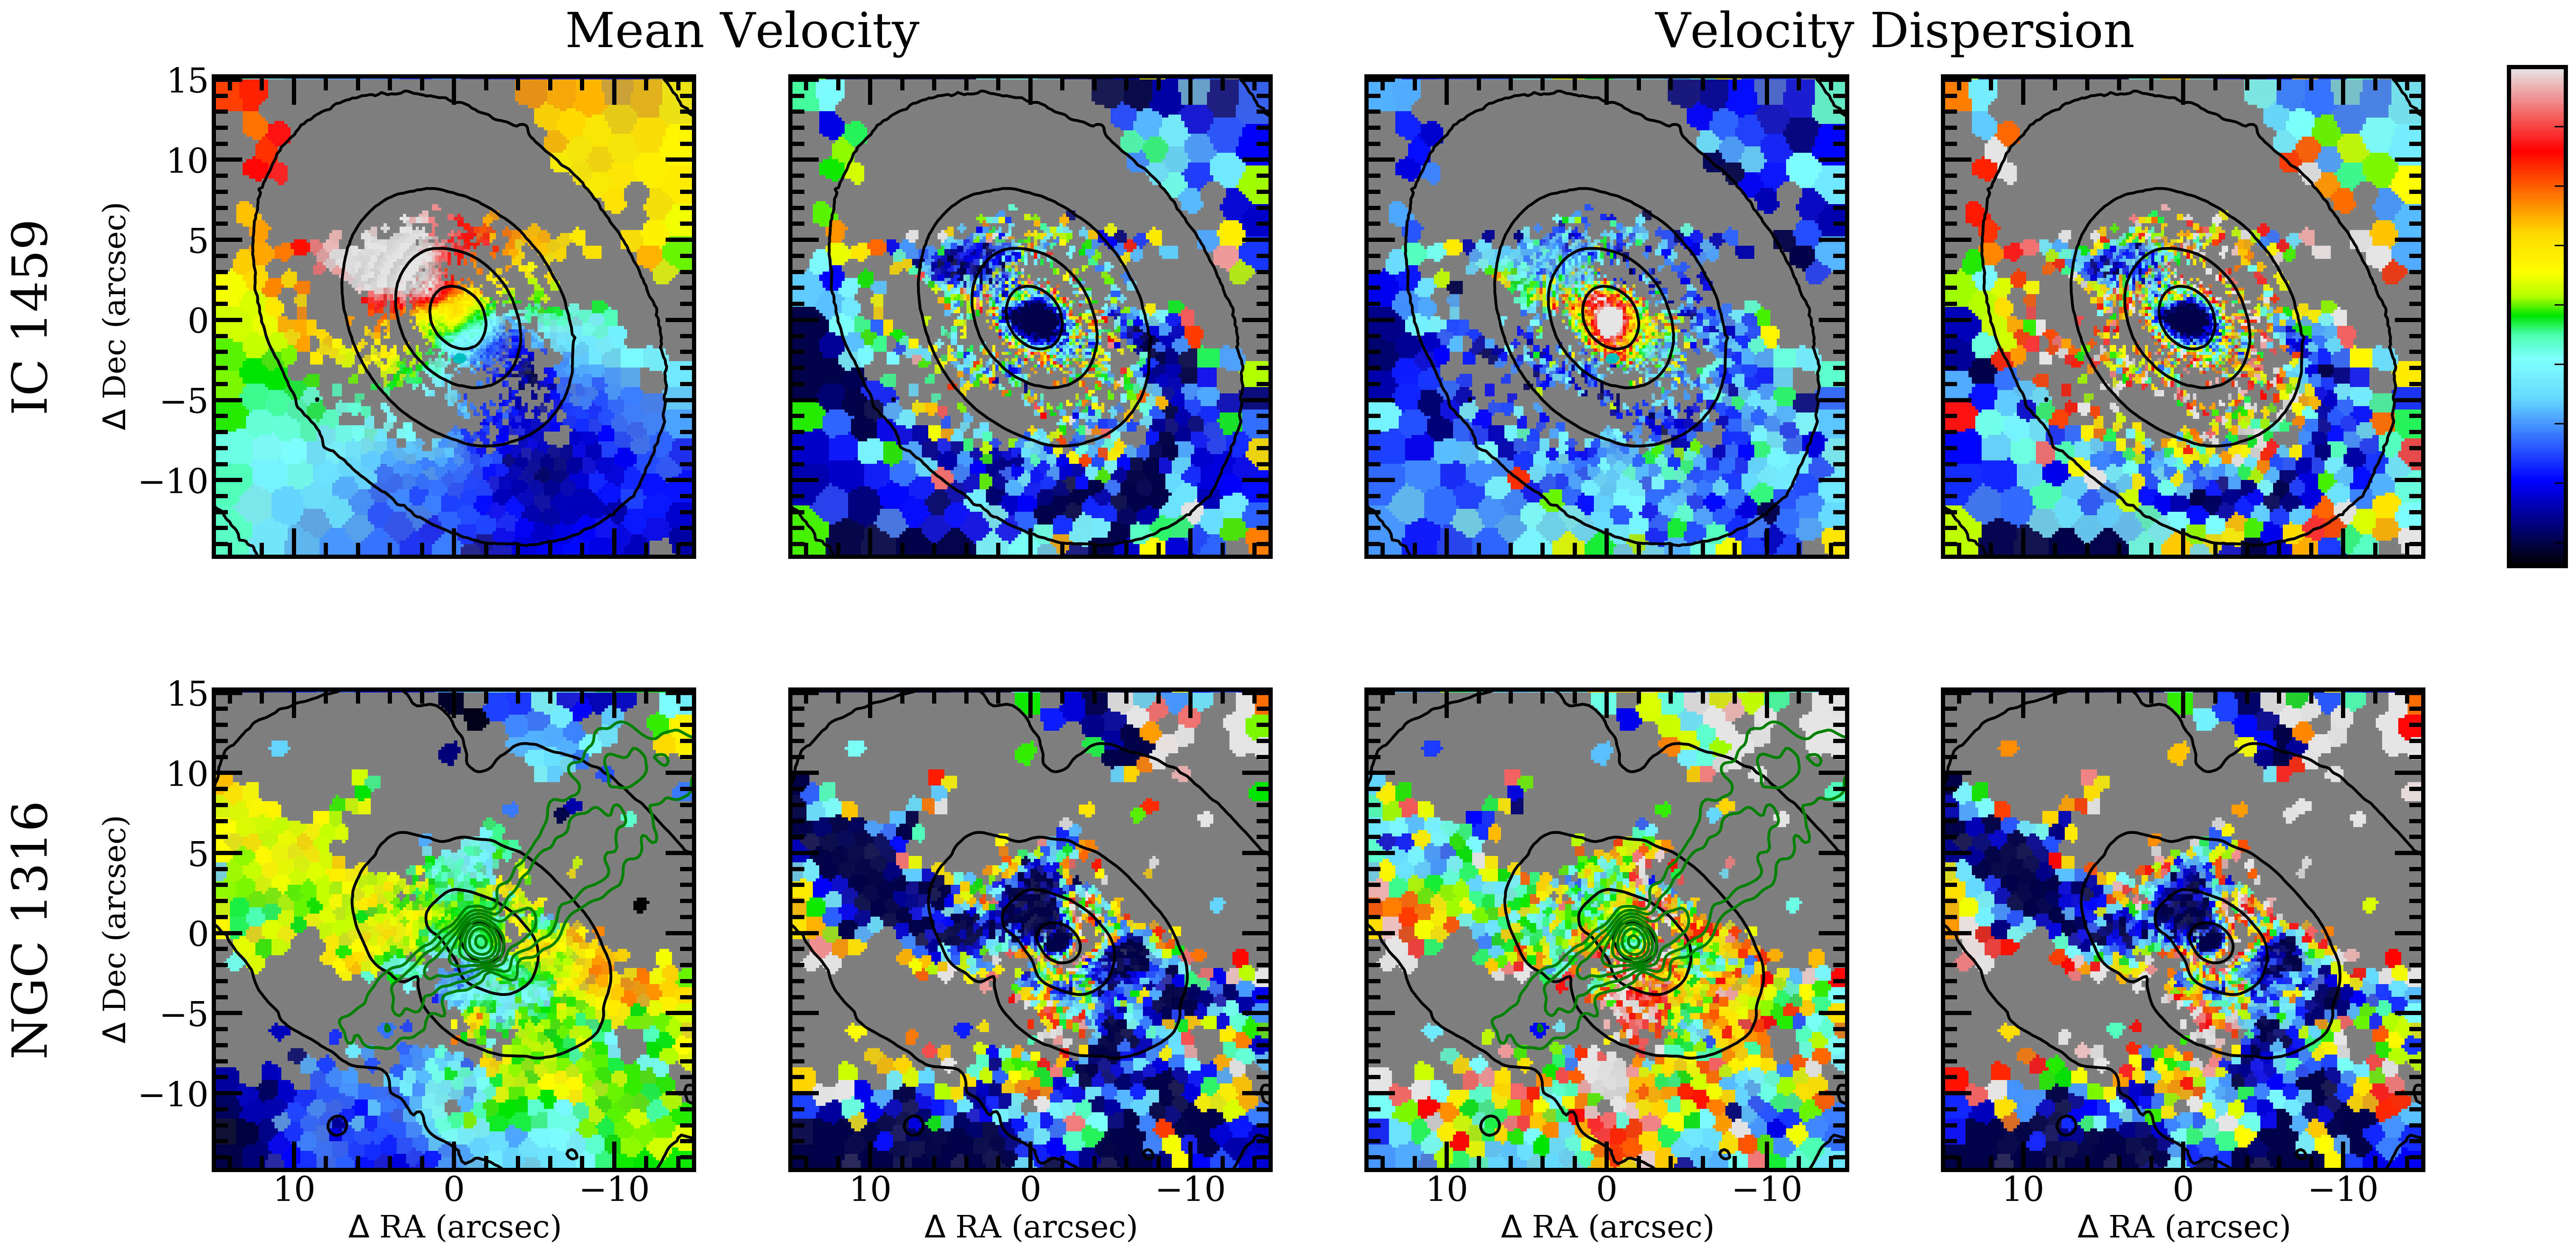
\includegraphics[height=0.31\textheight]{chapter5/muse/kin.png}
		\caption[MUSE ISM kinematic maps]{As in Figure \ref{fig:VIMOS_Gaskine} but for the MUSE ISM kinematic maps.}
		\label{fig:MUSE_Gaskine}
	\end{figure}


% Separate section?
	% \subsection{Misalignment of Gas}
	% 	\label{subsec:Gasmisaligment}
	It is immediately clear when comparing the mean stellar velocity maps in Figs.\,\ref{fig:VIMOS_stellar} and \ref{fig:MUSE_stellar} to the mean gas velocity maps in Figs.\,\ref{fig:VIMOS_Gaskine} and \ref{fig:MUSE_Gaskine} that where gas is detected, its angular momentum vector is not often aligned with that of the stars. A misalignment between kinematics of the stars and gas suggests and external origin to the gas (e.g. accretion or a wet merger), however it should be noted that the counter-argument is not necessarily true: aligned kinematics is \textit{only} consistent with an internal origin (e.g. stellar-mass loss), but does not require it \citep[e.g.][]{Davis2011a}. Here we address each of the four galaxies in turn. 

	\paragraph{IC 1459} shows the gas counter-rotating with respect to the kinematically-decoupled core, and is rotating independently from the rest of the galaxy too. Indeed the gas is rotating with a mean velocity which is an order of magnitude higher than that of the stars (outside of the KDC). It is unlikely that the gas in the progenitor galaxy to IC 1459 survived the merger event which created the KDC, given that the stellar disc did not survive. The lost gas may, however, have been re-accreted. Alternatively, the ISM may have a purely external origin. 

	\paragraph{NGC 612} has well aligned kinematics of the stars and gas. The misalignment between the position angle of the stellar and gas kinematics (using the method described in Section \ref{subsec:Misalignment}) is just $(1.0\pm0.7)$\,\degree. The lack of misalignment between the stellar and ionized gas kinematics is consistent with an internal origin for the gas. This adds to the evidence (see Section \ref{sec:NGC612}) that it has not undergone a major merger (major mergers tend to strip galaxies of their gas) and suggests that in the case of NGC 612, the fueling and powering of the radio jet must be a purely secular process. 


	\paragraph{NGC 1316} is a more complex case. The disc of gas in NGC 1316 is consistent with being aligned with the kinematics of stars, with a large inflow towards the nucleus from the south-west (See fig.\,\ref{fig:Inflow}). This inflow is almost perpendicular to the radio jet. However, we acknowledge that other interpretations are possible and longer exposure time is required to add certainty to this interpretation. However this map is interpreted it is clear that the gas in not in a settled disc. 

	\begin{figure}
		\centering
		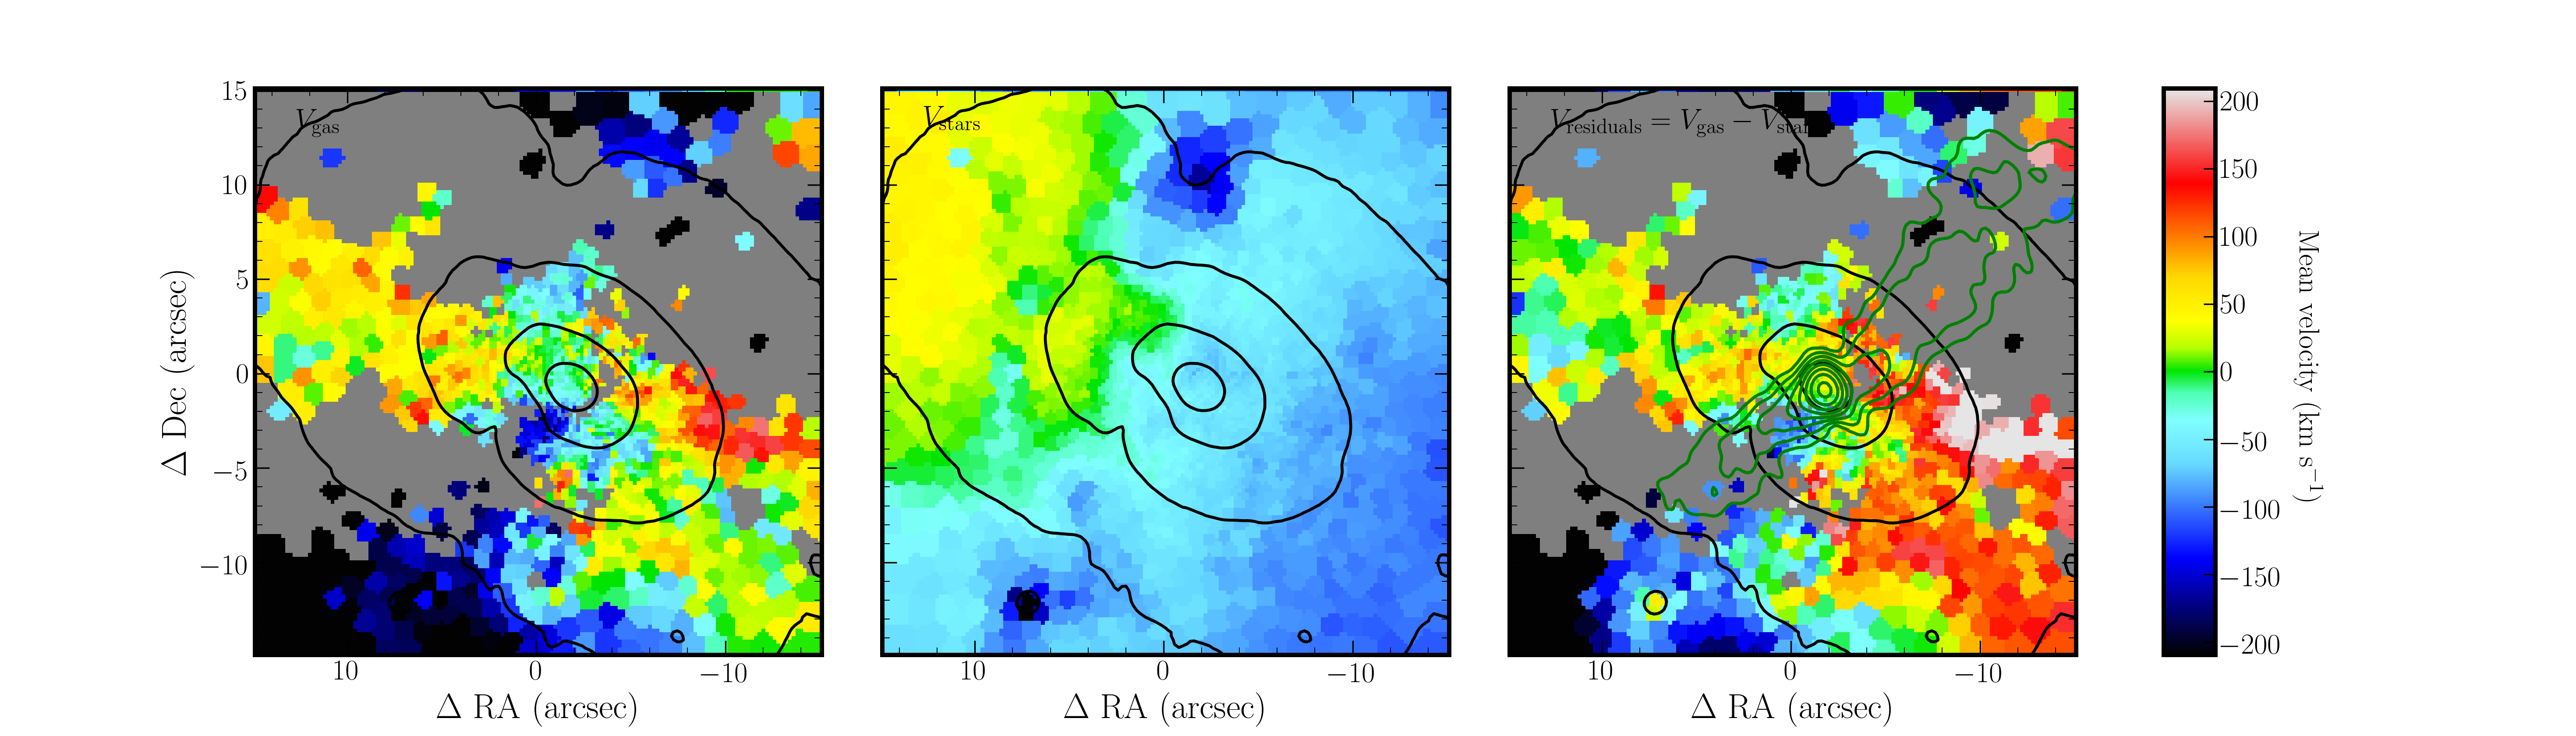
\includegraphics[width=\textwidth]{chapter5/ngc1316_inflow.png}
		\caption[Inflows in NGC 1316]{Inflows in NGC 1316.} 
		\label{fig:Inflow}
	\end{figure}


	\paragraph{NGC 3100} has an interesting morphology in the ISM. This \ce{^{12}CO(2-1)} contours (show in cyan in all figures) shows a broken ring shape with the radio jet passing through the gaps in the ring (Ruffa in prep.). We observe the ionised ISM to be brightest in the gaps of this ring. The simplest observation that we can make of the kinematics is that it is completely different to that of the stars. Secondly, that the centre of rotation of the gas appears to be offset from the centre of the galaxy (as defined by the surface brightness) by several arc-seconds to the west. 

	\citet{Davis2011a} show that ($36\pm5$)\% of fast rotators have misaligned ionized gas kinematics with respect to the stellar kinematics, while slow rotators have a flat distribution of misalignments. This indicates that slow rotators are dominated by external sources of gas, while fast rotators can have either. This is consistent with our observations of the Southern sample: the only slow rotator with detected ionized gas is IC 1459, which has significantly misaligned gas; while of the 3 fast rotators, only 1 (NGC 3100) is definitely misaligned. The other 2 galaxies (NGC 612 and NGC 1316) are therefore consistent with an internal origin to the gas.



\section{Sources of Ionising Potential}
	\label{sec:Diagnostics}
	Determining the source of the ionising radiation using line ratio plots, such as Baldwin--Phillips--Terlevich (BPT) plots (\citealt{Baldwin1981}; and revised by \citealt{Kewley2001, Kewley2006} and \citealt{Kauffmann2003a}), has become increasingly useful tool. That said, there are several important caveats. Firstly, great care must be taken in applying the definitions of each diagnostics line. Much of the literature mis-interprets the classifications. Secondly, in the absence of spatially resolved spectra, low-ionisation nuclear emission-line region (LINER) classifications have often been taken as a marker for jet-mode active galactic nuclei (AGN). As discussed in Section \ref{subsubsection:JetFeedback}, several recent surveys have shown that many of these galaxies may not be bona fide AGN \citep[e.g.][]{Sarzi2005, Sarzi2010, Singh2013, Belfiore2016a}. In such cases, the emission may not even originate from the centre of the galaxies, the location of the supposed AGN. This led to the creation of the low-ionisation emission-line region (LIER) classification, with the same criteria as LINER, but not necessarily in the nuclear region.

	The problem with classifying ETGs by their emission lines, is that they often have very little ionized gas and weak ionizing radiation fields. This means that it is difficult to detect emission lines from the ISM. Furthermore, the BPT plots require a larger spectral range than many integral field unit (IFU) instruments are equipped with. This has given rise to a number of other, similar, classifying plots, which we take advantage of here. A description of of our classifying process follows below. 

	Firstly, we preferentially use the BPT plots for the galaxies observed with MUSE (which has the required spectral range; see Section \ref{subsec:BPT}). This classifies galaxies into star-forming, LINER/LIER or Seyfert 2 classes. For the emission line strengths derived from VIMOS datacubes, we use the [\ion{N}{i}]/H\,$\beta$ verses [\ion{O}{iii}]/H\,$\beta$ plot from \citet[hereafter the SAURON plot]{Sarzi2010}. Unlike the BPT plots, \citet{Sarzi2010} do not define classifying lines. We use the Balmer decrement (see Section \ref{subsec:Ndec}) and the gradient of the [\ion{N}{i}] verse [\ion{N}{ii}] plot (Section \ref{subsec:Ndec}) to convert the classification lines of \citet{Kewley2001} and \citet{Kauffmann2003a} from the [\ion{N}{ii}]/H\,$\alpha$ BPT plot to the [\ion{N}{i}]/H\,$\beta$ SAURON plot (described in more detail in Section \ref{subsec:Ndec}). This classifies galaxies into star-forming or LINER/Seyfert 2 classes. We also use the so-called WHaN2 (H\,$\alpha$ equivalent width verses [\ion{N}{ii}]/H\,$\alpha$) plot (see Section \ref{subsec:WHaN2}) from \citet{CidFernandes2011}. Using the same method as above we translate this the H\,$\beta$ equivalent width verses [\ion{N}{i}]/H\,$\beta$ (WHbN1) plot for the VIMOS data. In order to transpose the equivalent widths from H\,$\alpha$ to H\,$\beta$ we find the average gradient of the continuum at the rest frame of H\,$\alpha$, $C_\text{6563\AA}$, plotted against the continuum at the rest frame of H\,$\beta$, $C_\text{4861\AA}$ (also described in more detail in Section \ref{subsec:Ndec}). This classifies galaxies into star-forming, strong AGN (Seyfert 2), weak AGN (LINER) or retired classes. In order to check if LINER classifications are due to a central radiation source (such as the AGN) or extended sources (such as weak star formation or post-asymptotic giant branch stars; pAGB stars), we examine the H\,$\alpha$ and H\,$\beta$ flux radial profiles for galaxies with extended detected gas for MUSE and VIMOS data, respectively (Section \ref{subsec:Hb}). Finally, in Section \ref{subsec:MEx} we use the mass--excitation (MEx) plot of \cite{Nyland2016} using only the derived parameters from the central region of the galaxies, measured with a 3$^{\prime\prime}$ wide aperture. This classifies into star-forming, Seyfert 2, LINER, transition or passive classes, with LINER galaxies subdivided into those whose LINER behavior is attributed to a central AGN (LINER-AGN) and those that cannot. 


	\subsection{Using Emission Lines Beyond the Range of VIMOS Data}
		\label{subsec:Ndec}

		The Balmer decrement, $d_\mathrm{H}$, is the ratio of the H$\alpha$ to H$\beta$ fluxes and has good theoretical motivation that it has a near constant value of $d_\mathrm{H} = 2.86$ under a wide variety of conditions. In reality, however, higher values are routinely observed. These observation can be explained as either due to the presence of dust, causing extinction, whereby emission lines at longer wavelengths to appear brighter than expected compared the their bluer counterparts as the dust preferentially scatters bluer light; or some mechanism that populates hydrogen levels from the ground up. Such mechanisms may be important in high-density environments such at within powerful (type 1) AGN nuclei \citep[e.g.][]{Shields1974, Netzer1975}. The majority ($\approx 60$\%) of ETGs and all low-ionized nuclear emission region galaxies (LINERs) and Seyfert galaxies are dusty in nature \citep[e.g.][]{Martini2013}. Such galaxies have clear dust observations in \textit{Hubble Space Telescope (HST)} observations \citep[e.g.][]{Martini2013}, are bright in the infrared (where the thermal emission from dust is seen in the `dust bump'; e.g. \citealt{Jura1987, Knapp1992}) and other emission line ratios \citep[e.g. \bracket{\ion{S}{ii}} in ][]{Wampler1968} show similar reddening. Thus, assuming the observed steeping of the Balmer decrement is entirely due to dust, the ratio of the observed decrement to the theoretical value of 2.86 is a good estimate for the reddening effect of the dust.

		If we assume that different ionization states of a given atom occur in the same locations (namely, the location of the abundance of the atom), implying that shielding is not important or at least is not non-linear in its affect on the emission-line ratios. Given that the different species must have been produced under the same conditions, it might be natural to expect a relationship between them. Thus, using the emission line fluxes derived from the MUSE data, we observe that the relationship between [\ion{N}{ii}] and [\ion{N}{i}] appears to be linear. We emphasis that these are purely empirical observations and differ from the Balmer decrement as they lack strong theoretical basis. 

		In order find the intrinsic conversion from [\ion{N}{i}] to [\ion{N}{ii}] we must first correct for dust reddening. Assuming that the extinction can be approximated to a linear form in the V-band, we correct the flux of the bluer emission line, $I_\mathrm{b}$ of the pair by applying
		\begin{equation}
			I^\mathrm{corr}_\mathrm{b} = I_\mathrm{b} \frac{\Delta\lambda}{\lambda_\mathrm{H\alpha} - \lambda_\mathrm{H\beta}} \frac{I_\mathrm{H\alpha}}{2.86 I_\mathrm{H\beta}} \, ,
		\end{equation}
		where $\Delta\lambda$ is the difference in wavelength of the two lines, $\lambda_\mathrm{H\alpha}$ and $\lambda_\mathrm{H\beta}$ are the rest-frame wavelengths of the H$\alpha$ (6563 \AA) and H$\beta$ (4861 \AA) emission lines with intensities of $I_\mathrm{H\alpha}$ and $I_\mathrm{H\beta}$, respectively. The intrinsic conversion can then be found by comparing $I^\mathrm{corr}_\mathrm{b}$ to $I_\mathrm{r}$, the intensity of the redder line in the pair. 

		In Fig.\,\ref{fig:NII_NI} we fit a straight line to the intensity of [\ion{N}{ii}] verse [\ion{N}{i}] corrected for dust extinction using the least-trimmed squares routine, \textsc{lts\_linefit} by \citet{Cappellari2013} due to its robust handling of uncertainty in both axes. As can be seen in the figure, there two galaxies have quite different gradients. We require a single function in order to be able to use [\ion{N}{i}] as a proxy for [\ion{N}{ii}] for our VIMOS data. We thus fit each galaxy independently and use the mean gradient, neglecting the intercept. We find a mean gradient of $12.23 \pm 0.14$.

		\begin{figure}
			\centering
			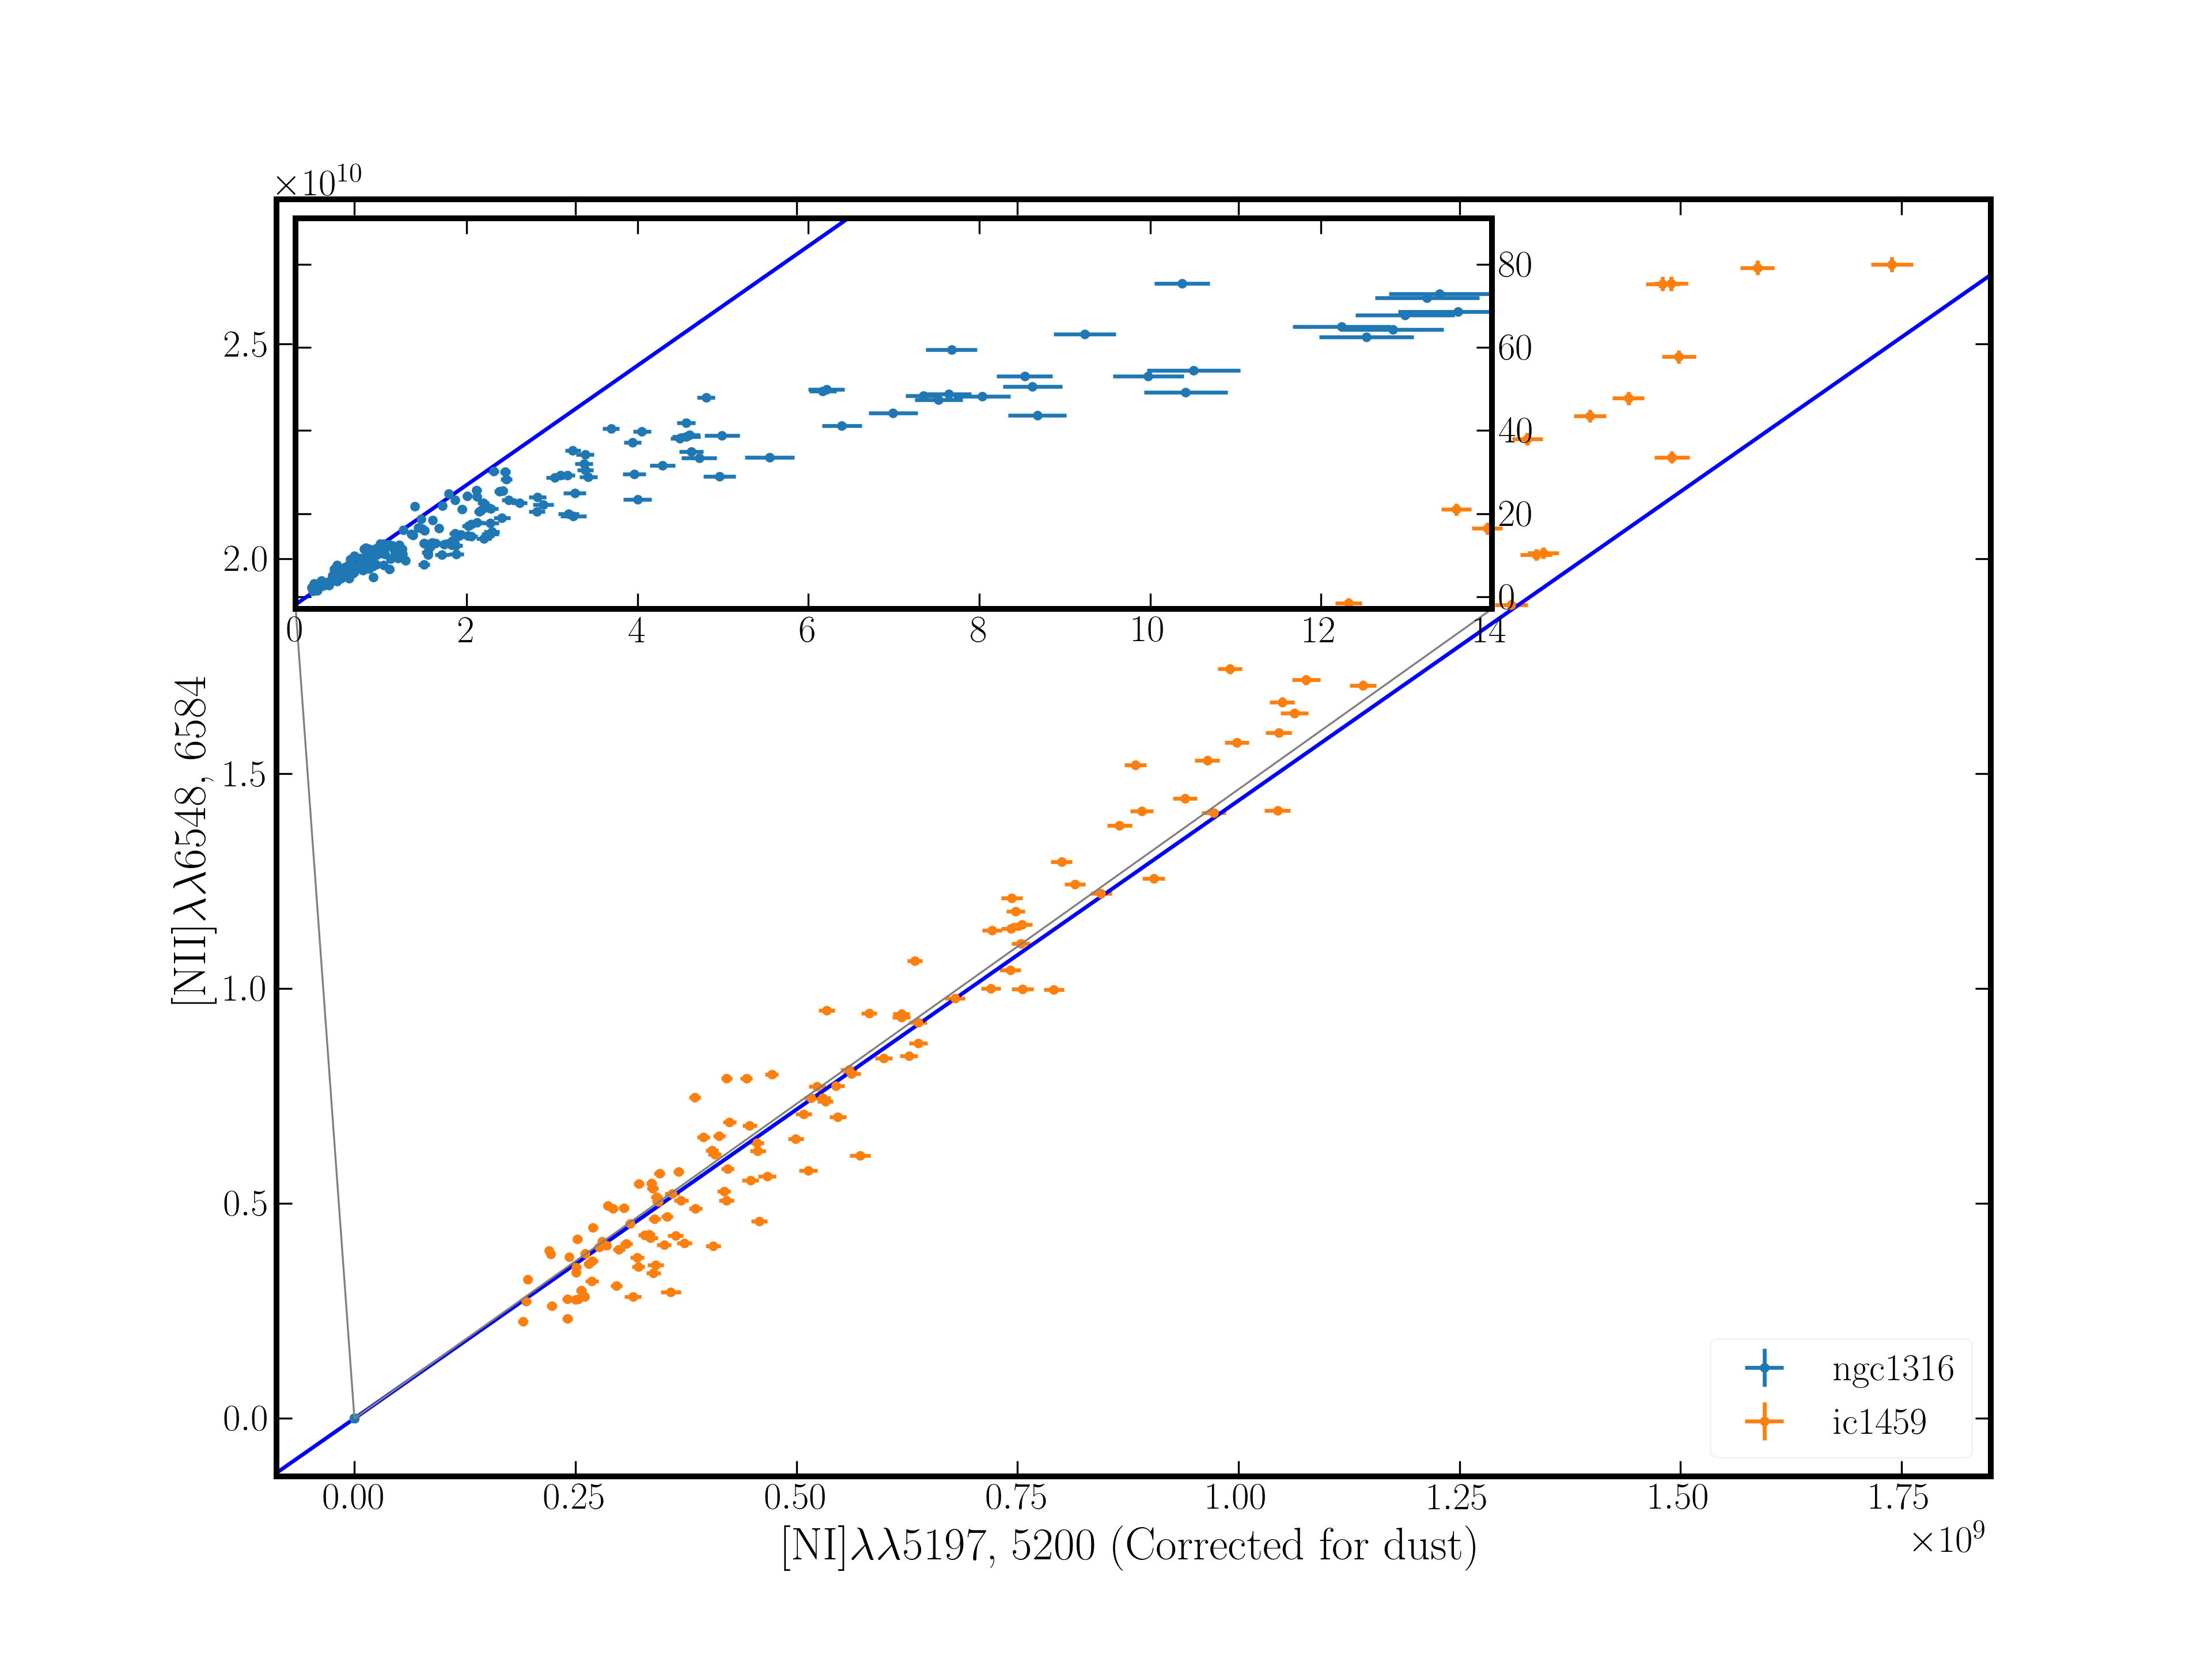
\includegraphics[width=0.7\textwidth]{chapter5/NII_NI_ratio.png}
			\caption[The nitrogen `decrement']{The Nitrogen `decrement': the gradient of the [\ion{N}{ii}] verses [\ion{N}{i}] plot for transposing classification lines of line ratios involving [\ion{N}{ii}] to [\ion{N}{i}]. In order to compare the 2 galaxies, the fluxes have also been corrected for each galaxy's distance (using their associated redshifts from Table \ref{tab:sample}).} 
			\label{fig:NII_NI}
		\end{figure}

		% Some of the brightest bins in Figs.\,\ref{fig:NII_NI} and \ref{figLOI_OIII} deviate away from the best-fitting line, with an excess in the bluer line. Given that these bins are located at the centre of the galaxy, we suggest that we are possibly over correcting for dust in these regions and that some of the reddening for the Balmer decrement is actually due to the different conditions close to the AGN. 

		In order to use the H\,$\beta$ equivalent width instead of the H\,$\alpha$ equivalent width, we require not only the Balmer decrement, but also the stellar `decrement' i.e. the ratio of the continuum level at H\,$\alpha$ to the continuum level at H\,$\beta$ wavelengths. In the same way as we did for the nitrogen `decrement', in Fig.\,\ref{fig:stellarDec} we find a linear relationship between the continuum level at 6563\,\AA, $C_\text{6563\AA}$, and the continuum level corrected for dust at 4861\,\AA, $C^\text{corr}_\text{4861\AA}$, in the MUSE data. Using Fig.\,\ref{fig:stellarDec}, we find
		\begin{equation}
			C_\text{6563\AA} = \, (1.047\pm0.008) C^\text{corr}_\text{4861\AA} + (0.142+/-0.004757) \times 10^{-6} \, .
		\end{equation}
		This is used to be able to adjust the classifying lines for when they are dependent on the equivalent width of H\,$\alpha$. 

		\begin{figure}
			\centering
			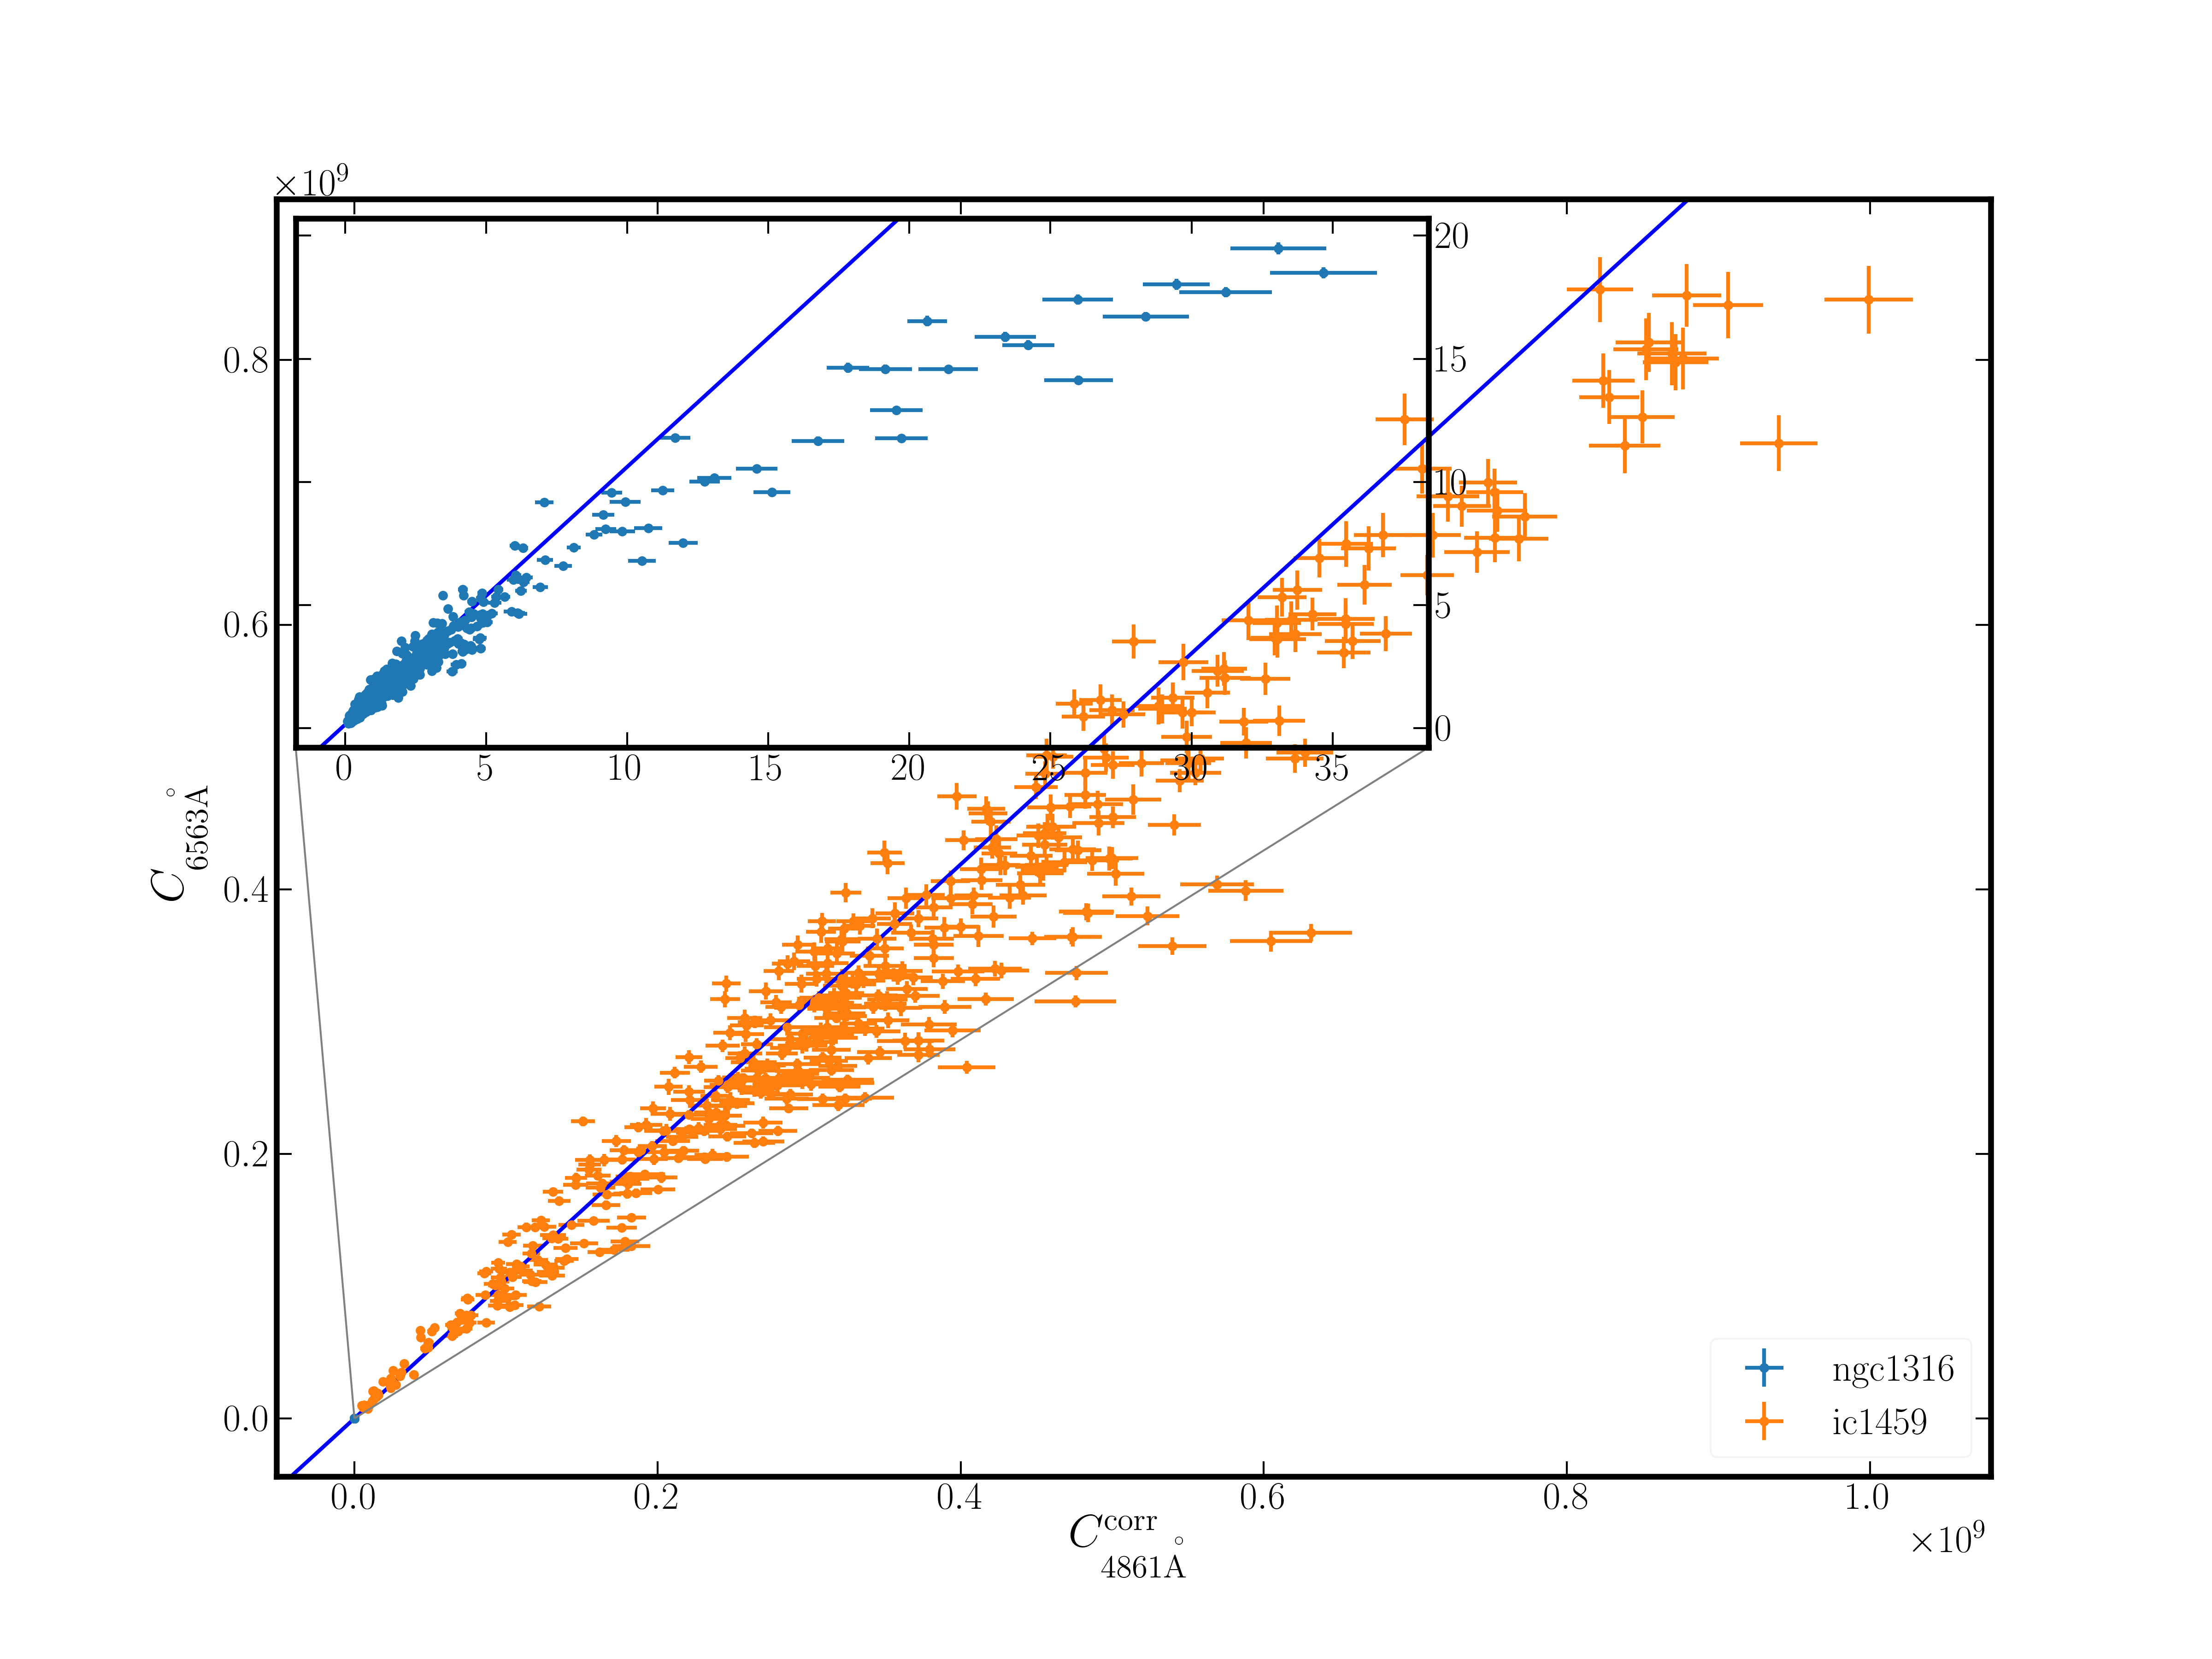
\includegraphics[width=0.7\textwidth]{chapter5/stellar_ratio.png}
			\caption[The stellar `decrement']{The stellar `decrement': the gradient of the continuum between H\,$\alpha$ and H\,$\beta$ rest frame wavelengths for transposing classification lines from H\,$\alpha$ to H\,$\beta$ equivalent widths. As in Fig.\,\ref{fig:NII_NI} these fluxes have been corrected for each galaxy's distance.} 
			\label{fig:stellarDec}
		\end{figure}

	\subsection{BPT Diagnostic Plots}
		\label{subsec:BPT}
		Firstly, in Fig.\,\ref{fig:BPT}, we examine our galaxies using the BPT diagnostic plots. Clearly for the traditional plots of [\ion{N}{ii}]/H\,$\alpha$, [\ion{S}{ii}]/H\,$\alpha$ and [\ion{O}{i}]/H\,$\alpha$ verses [\ion{O}{iii}]/H\,$\beta$, we can only use emission-line fluxes derived from the MUSE datacubes since the lines necessary for gauging the hardness of the ionizing radiation field are outside of the spectral range of VIMOS. Only two galaxies have detections of the necessary emissions line: IC 1459 and NGC 1316. Both occupy very similar positions on the BPT plots, on or close to the boundary between Seyfert 2 and LINER classifications. On the whole the central bins tend to be on the LINER side.

		\begin{figure}
			\centering
			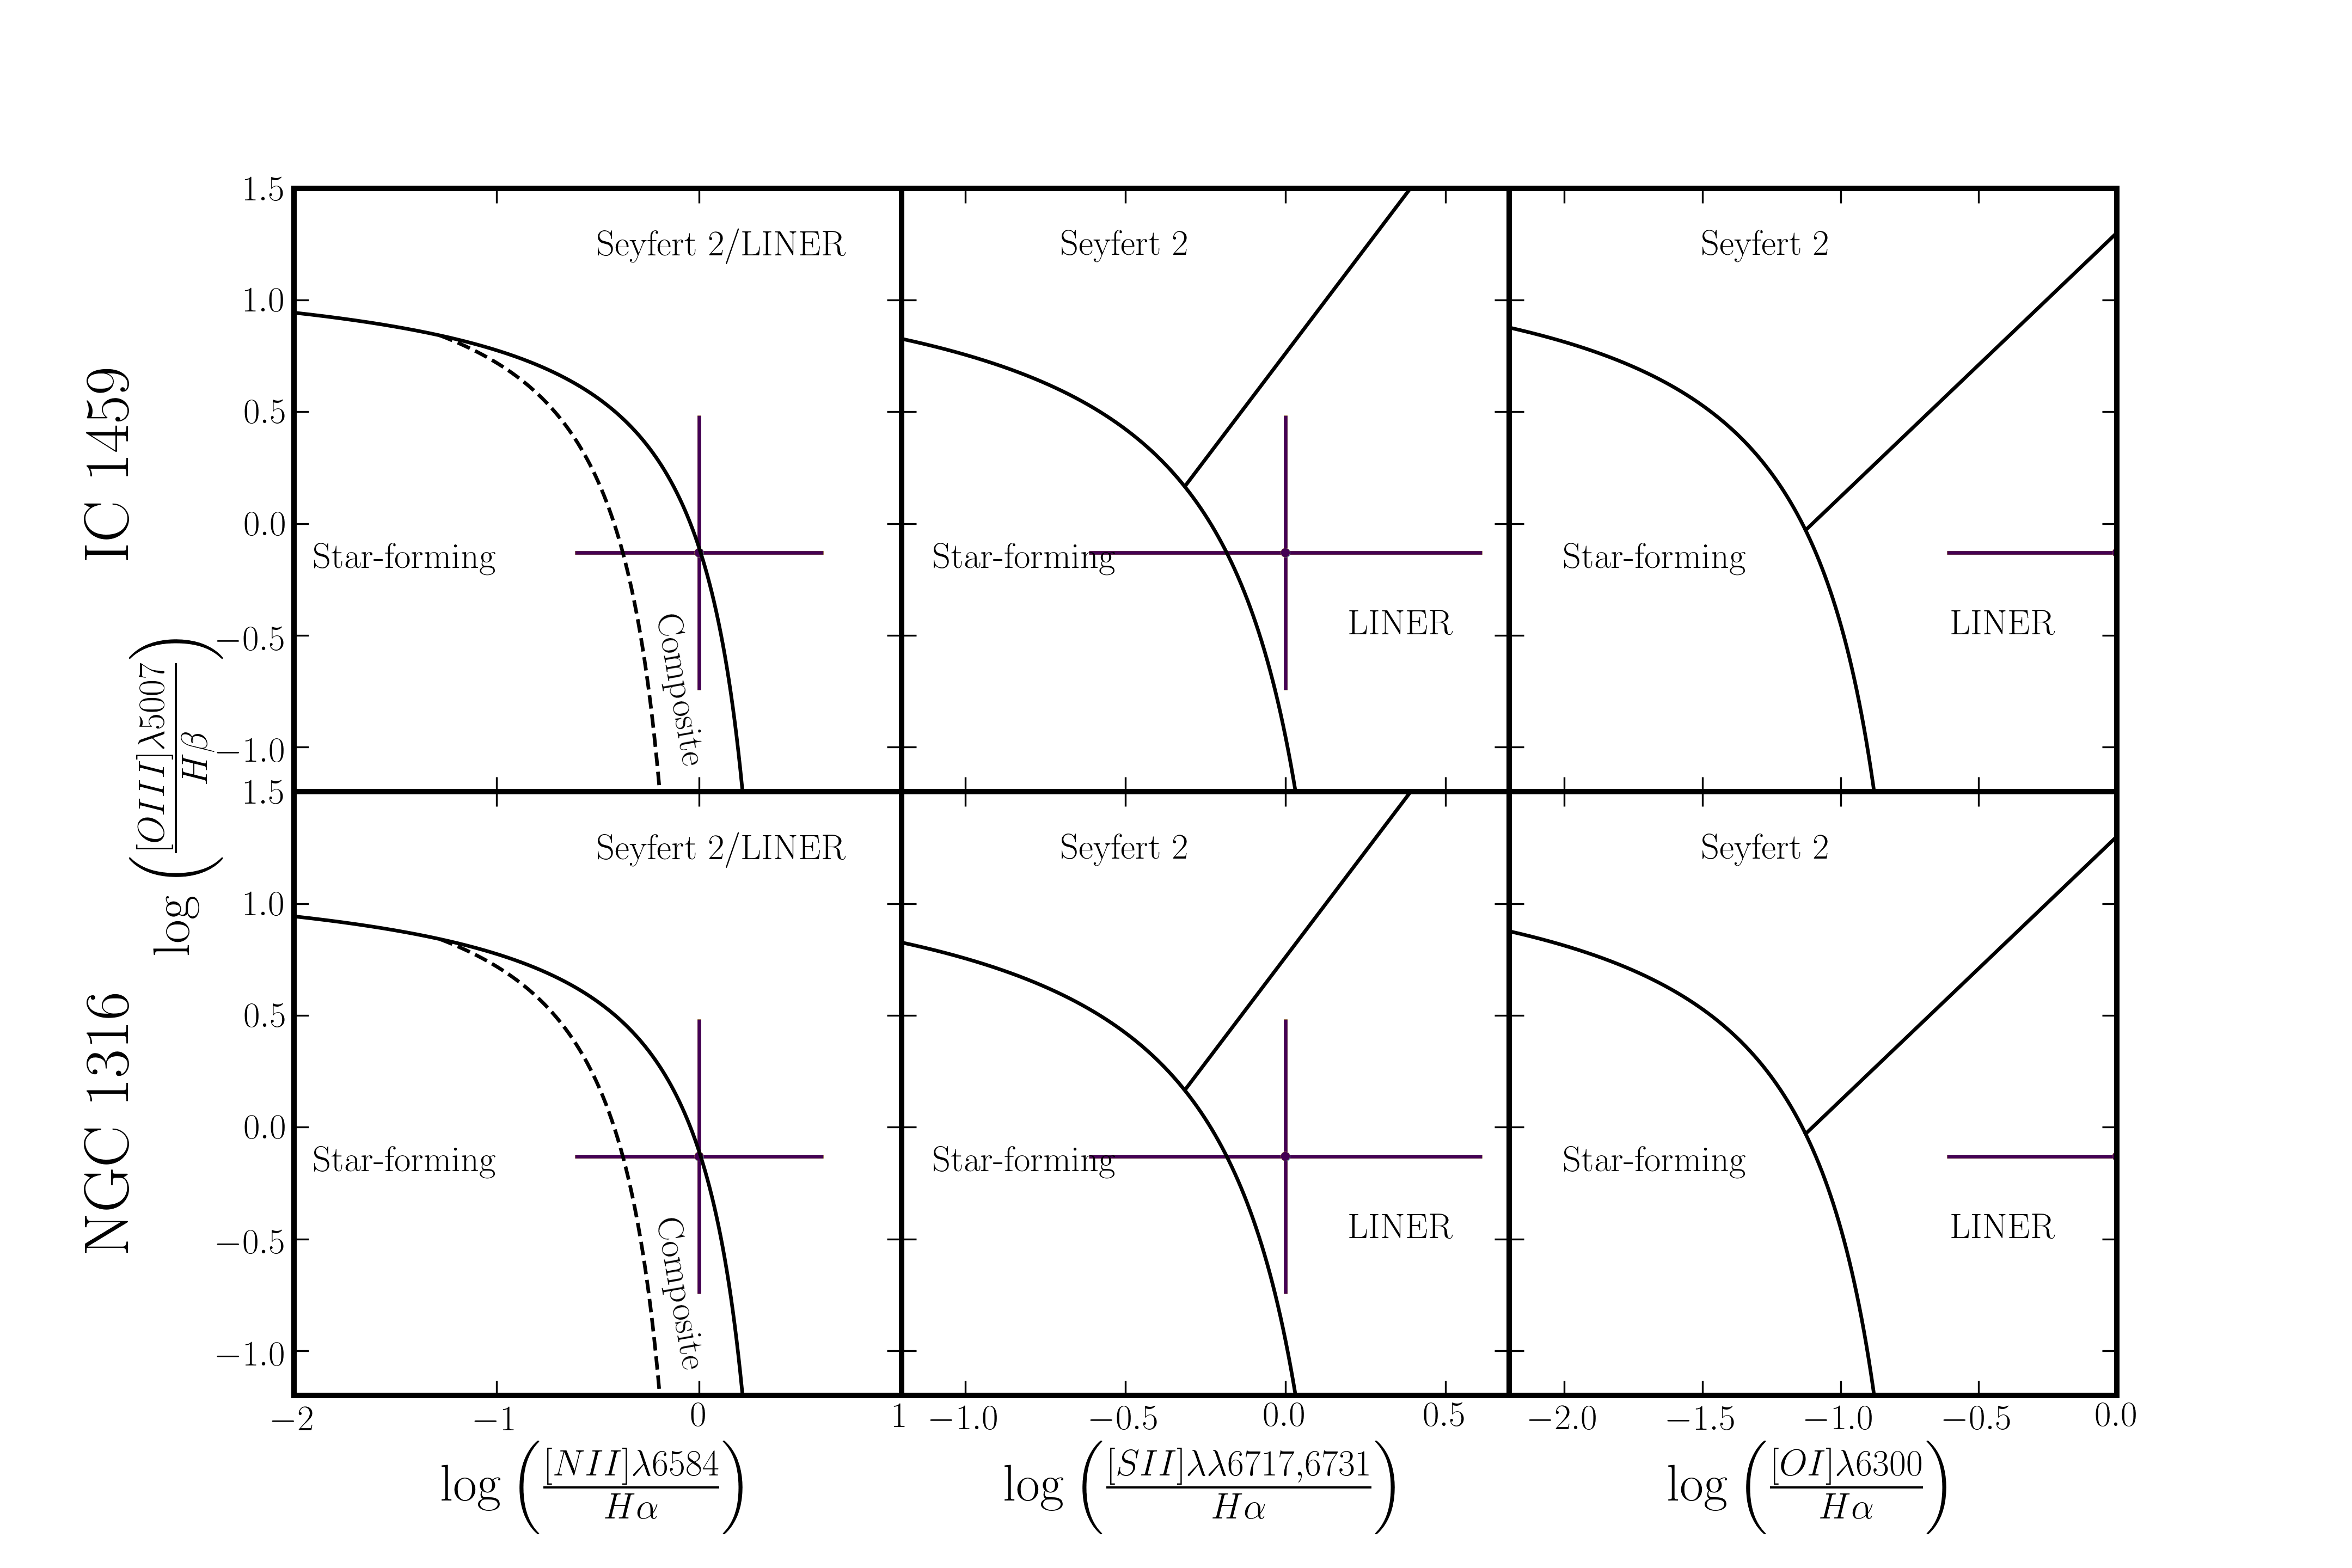
\includegraphics[width=\textwidth]{chapter5/BPT.png}
			\caption[BPT plots]{BPT plots for IC 1459 and NGC 1316. The colour scale (blue to yellow) represents increasing distance from the centre of the galaxy. The classification lines are from \citet{Kewley2006}.}
			\label{fig:BPT}
		\end{figure}

		\citet{Sarzi2010} show that Seyferts, LINERs and star-forming galaxies are reasonable separated in the [\ion{N}{i}]/H\,$\beta$ verses [\ion{O}{iii}]/H\,$\beta$ plot (hereafter the SAURON plot). We use the [\ion{N}{ii}] to [\ion{N}{i}] gradient (found in Section \ref{subsec:Ndec}) along with the Balmer decrement to transpose the \citet{Kewley2001} extreme starburst and \citet{Kauffmann2003a} pure star formation lines from the [\ion{N}{ii}]/H\,$\alpha$ verse [\ion{O}{iii}]/H\,$\beta$ plot to the SAURON plot.

		For the MUSE derived maps, only IC 1459 and NGC 1316 have detections of [\ion{N}{i}]. Given that we already have the superior BPT plots for these galaxies, we only show the VIMOS derived maps. These are shown in Fig.\,\ref{fig:SAURON}. All 6 galaxies with detectable emission lines within our binning system show AGN/LINER behavior.

		\begin{figure}
			\centering
			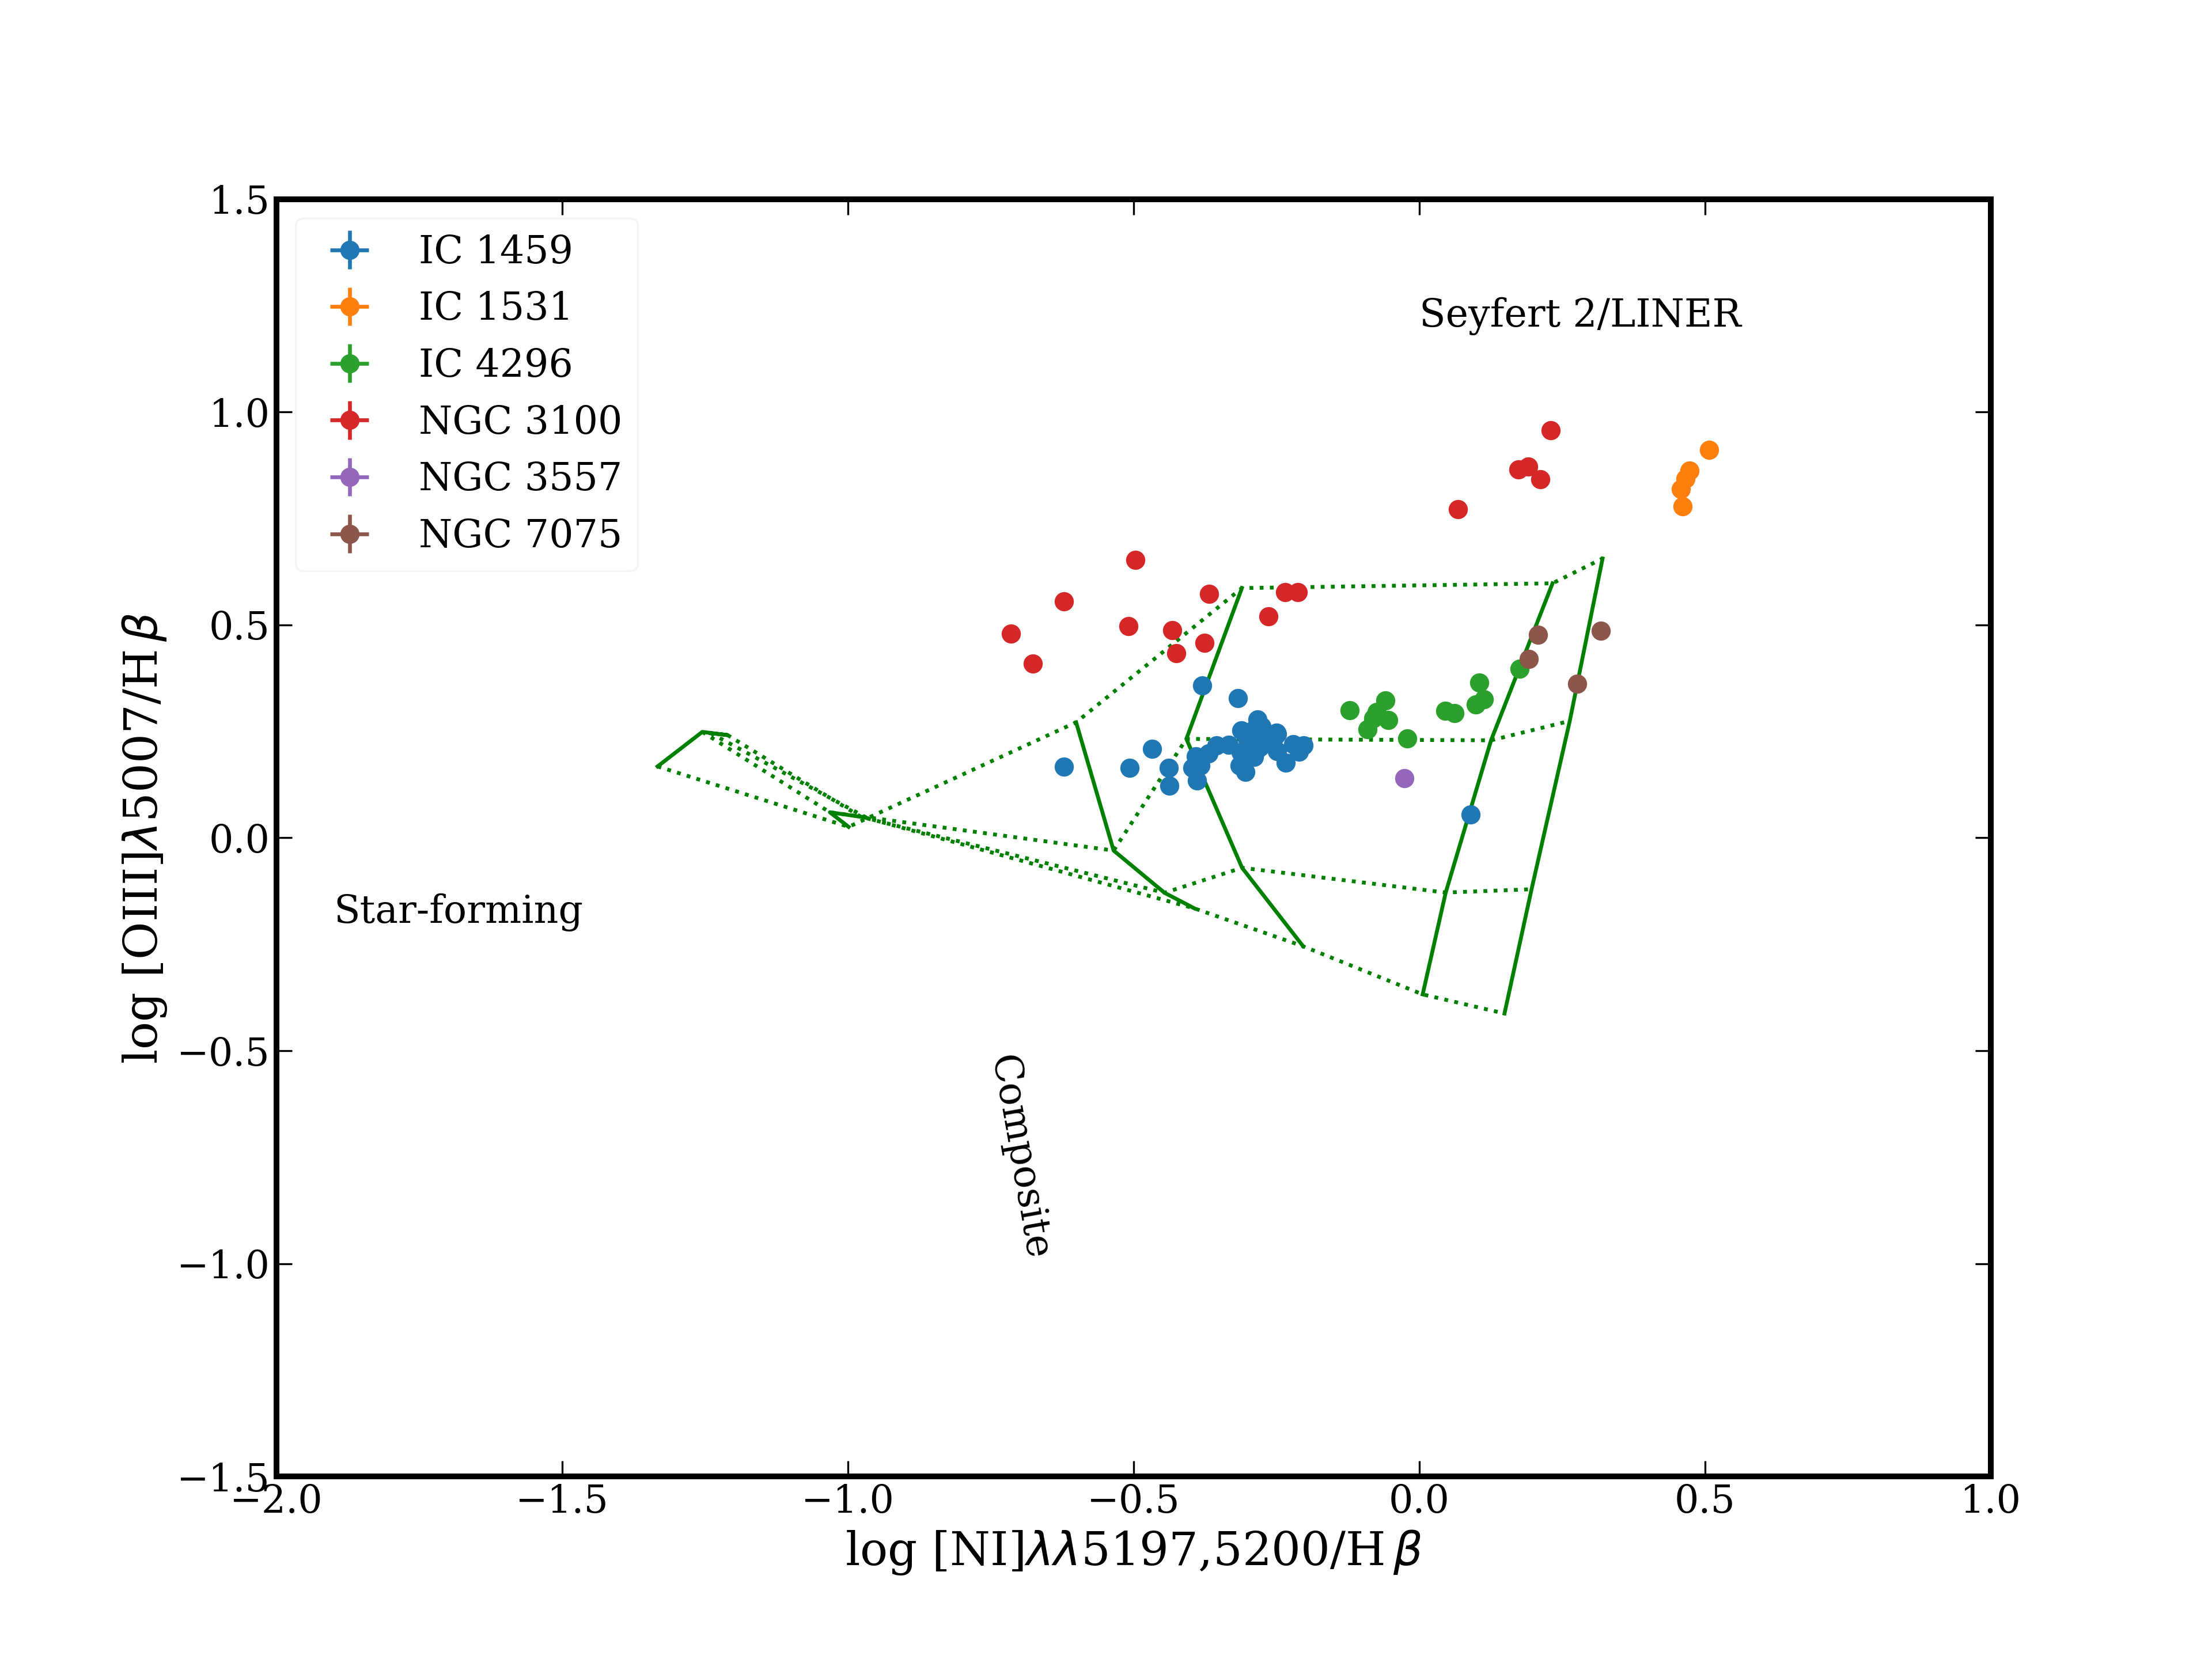
\includegraphics[width=0.8\textwidth]{chapter5/SAURON.png}
			\caption[An alternative diagnostic plot]{SAURON plot for line ratios from VIMOS datacubes. In order to show the expected LINER position on the SAURON plot, the green grid is the MAPPINGS-III models for shocks from \citet{Allen2008}. The solid lines are at constant shock velocities (from 150 to 1000\,$\mathrm{km\,s^{-1}}$) and the dotted lines constant magnetic parameter $b = B/\sqrt(n)$ (from 0.5 to 4.0), where B is the magnetic field strength and n is the (pre-shock) particle number density \citep{Dopita1996}. All models assume an electron density of $N_e = 1\,\mathrm{cm^{-3}}$.}
			\label{fig:SAURON}
		\end{figure}


	\subsection{WHaN2 Plots}
		\label{subsec:WHaN2}
		The final resolved line ratio plot that we use is the equivalent width of H\,$\alpha$ verses log [\ion{N}{ii}]/H\,$\alpha$. This is known as the WHaN2 plot. In Fig.\,\ref{fig:WHaN2} we show the WHaN2 plot for the MUSE derived emission lines for IC 4296. We do not include IC 1459 and NGC 1316 since they have already been classified via the standard BPT plots (see Section \ref{subsec:BPT}). We interpret a weak AGN classification as LINER-AGN.

		\begin{figure}
			\centering
			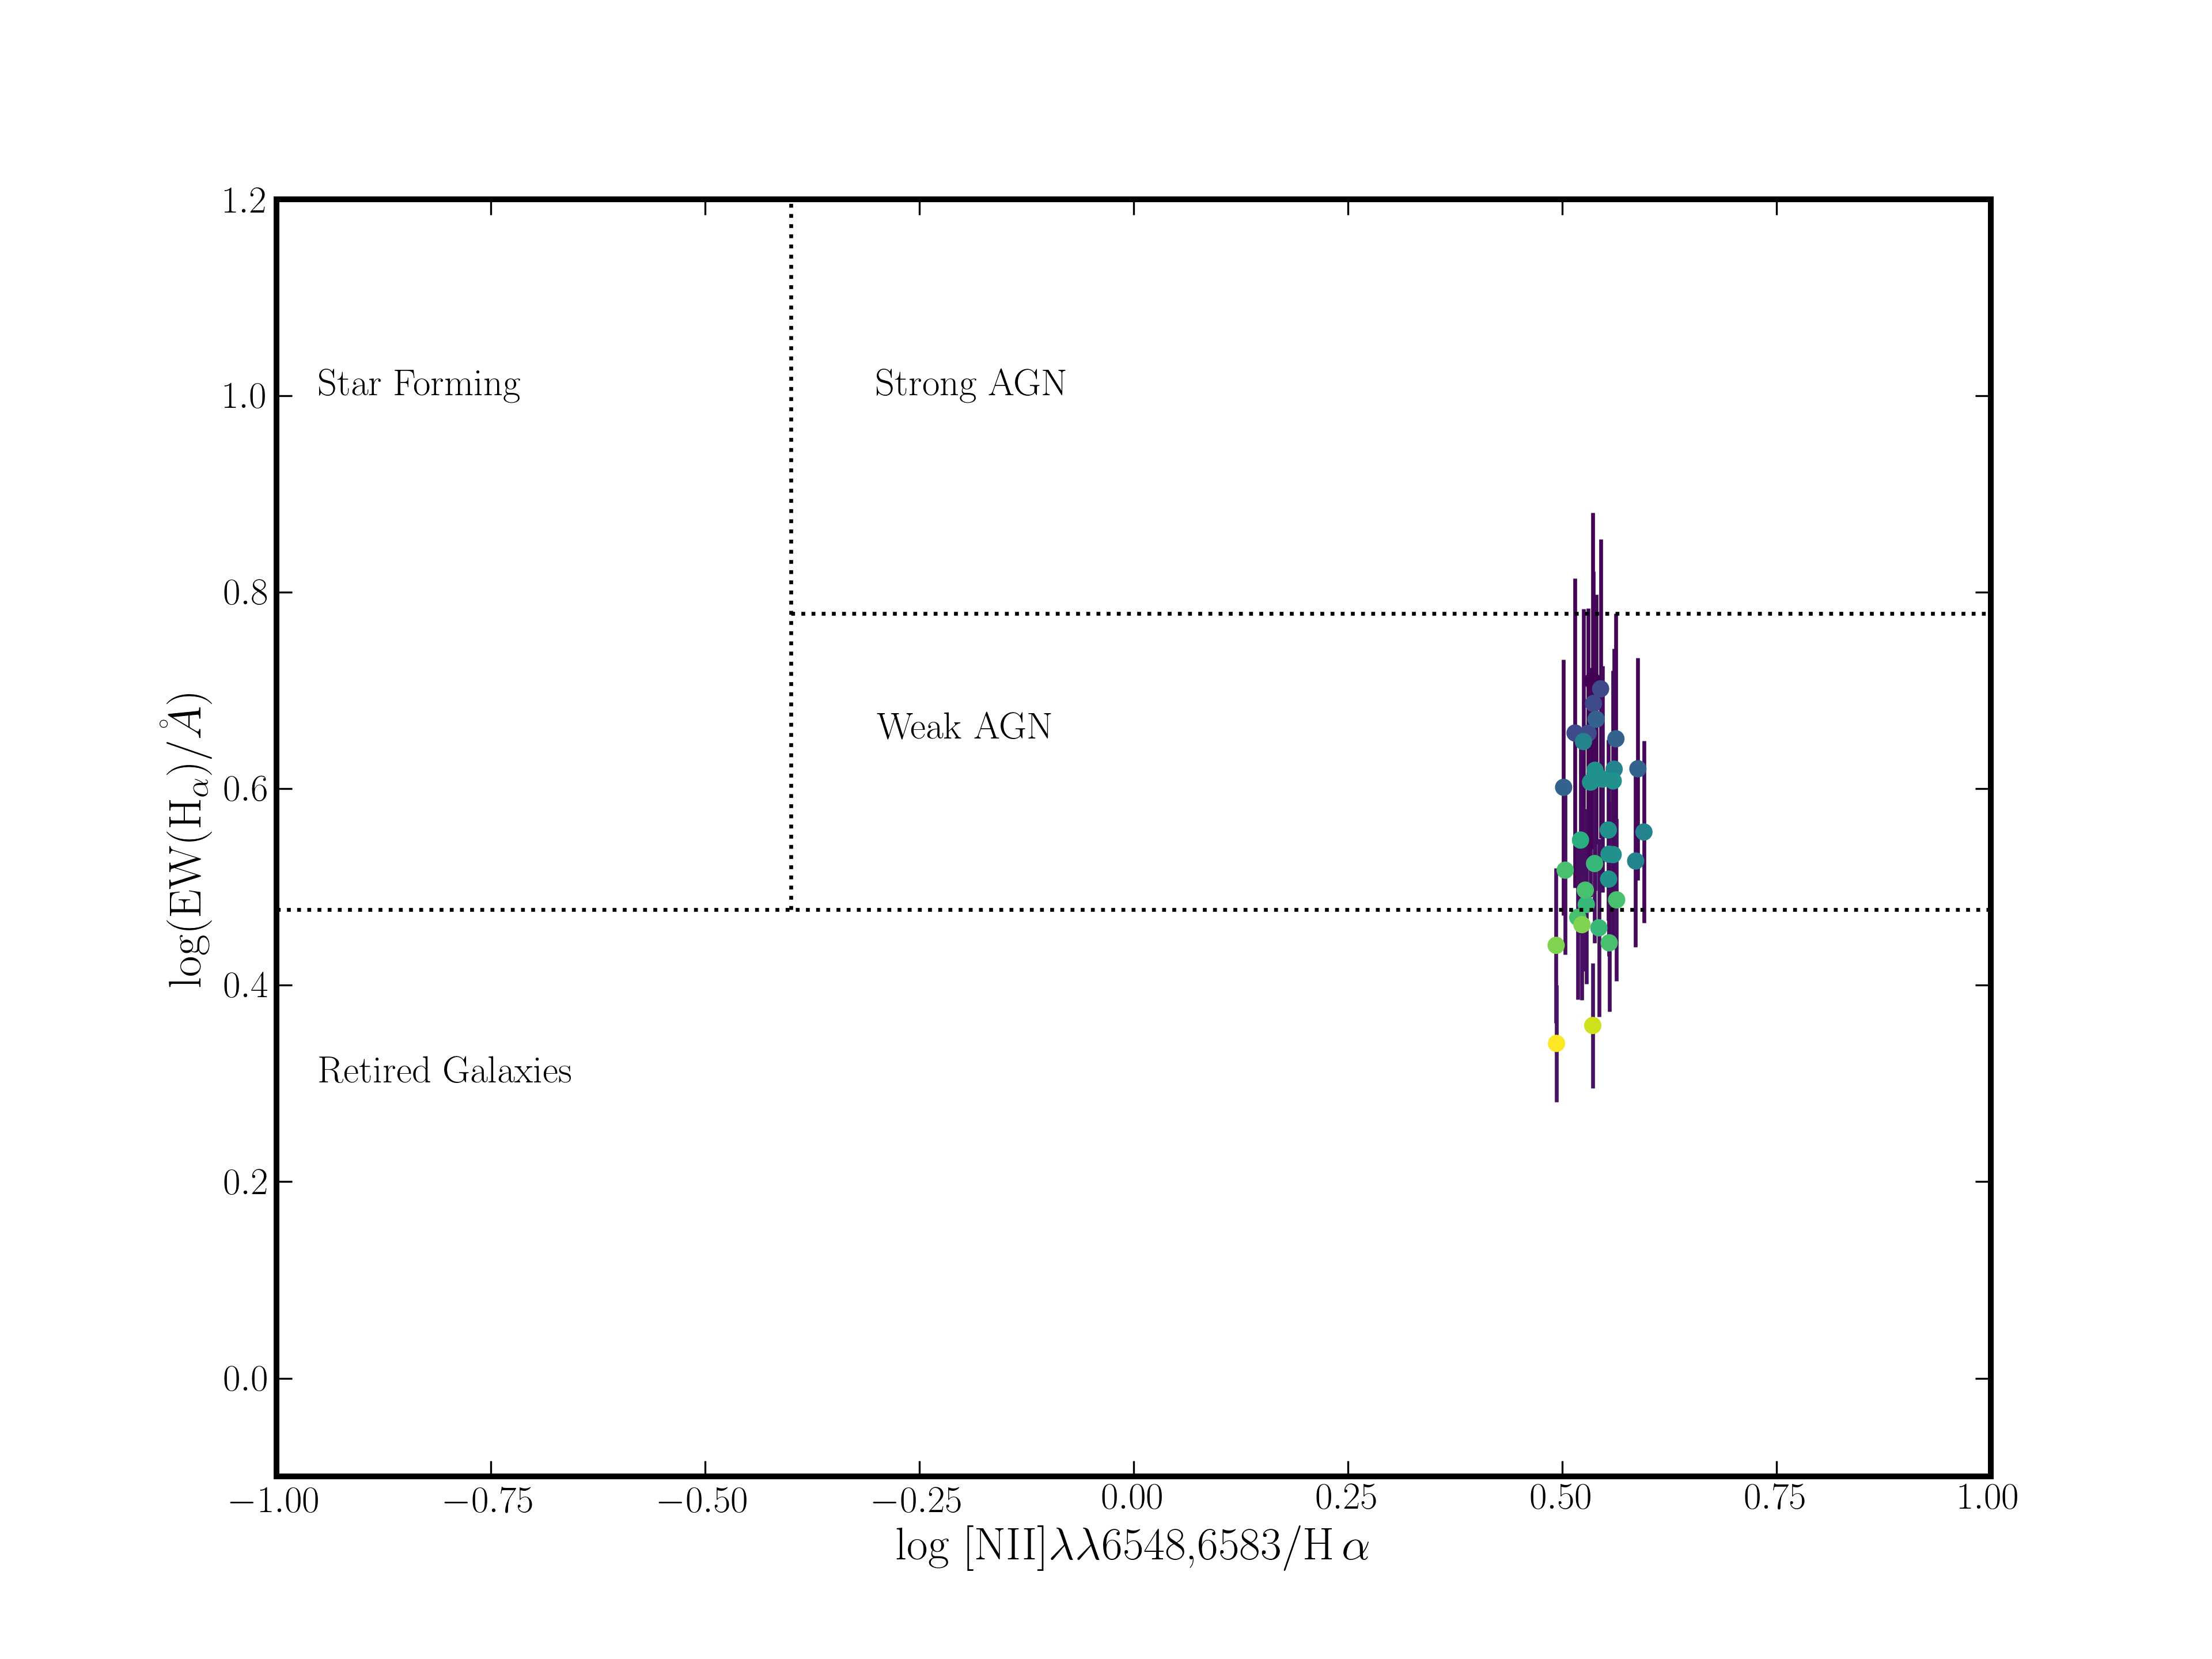
\includegraphics[width=0.8\textwidth]{chapter5/WHaN2.png}
			\caption[WHaN2 plot for IC 4296]{WHaN2 plot for IC 4296. The colour scale (blue to yellow) represents increasing distance from the centre of the galaxy.}
			\label{fig:WHaN2}
		\end{figure}


		For the emission lines derived from VIMOS datacubes we use H\,$\beta$ as a proxy for H\,$\alpha$ and [\ion{N}{i}] as a proxy for [\ion{N}{ii}] using the Balmer, nitrogen and stellar `decrements' to translate the classification lines. We call this the WHbN1 plot.

		\begin{figure}
			\centering
			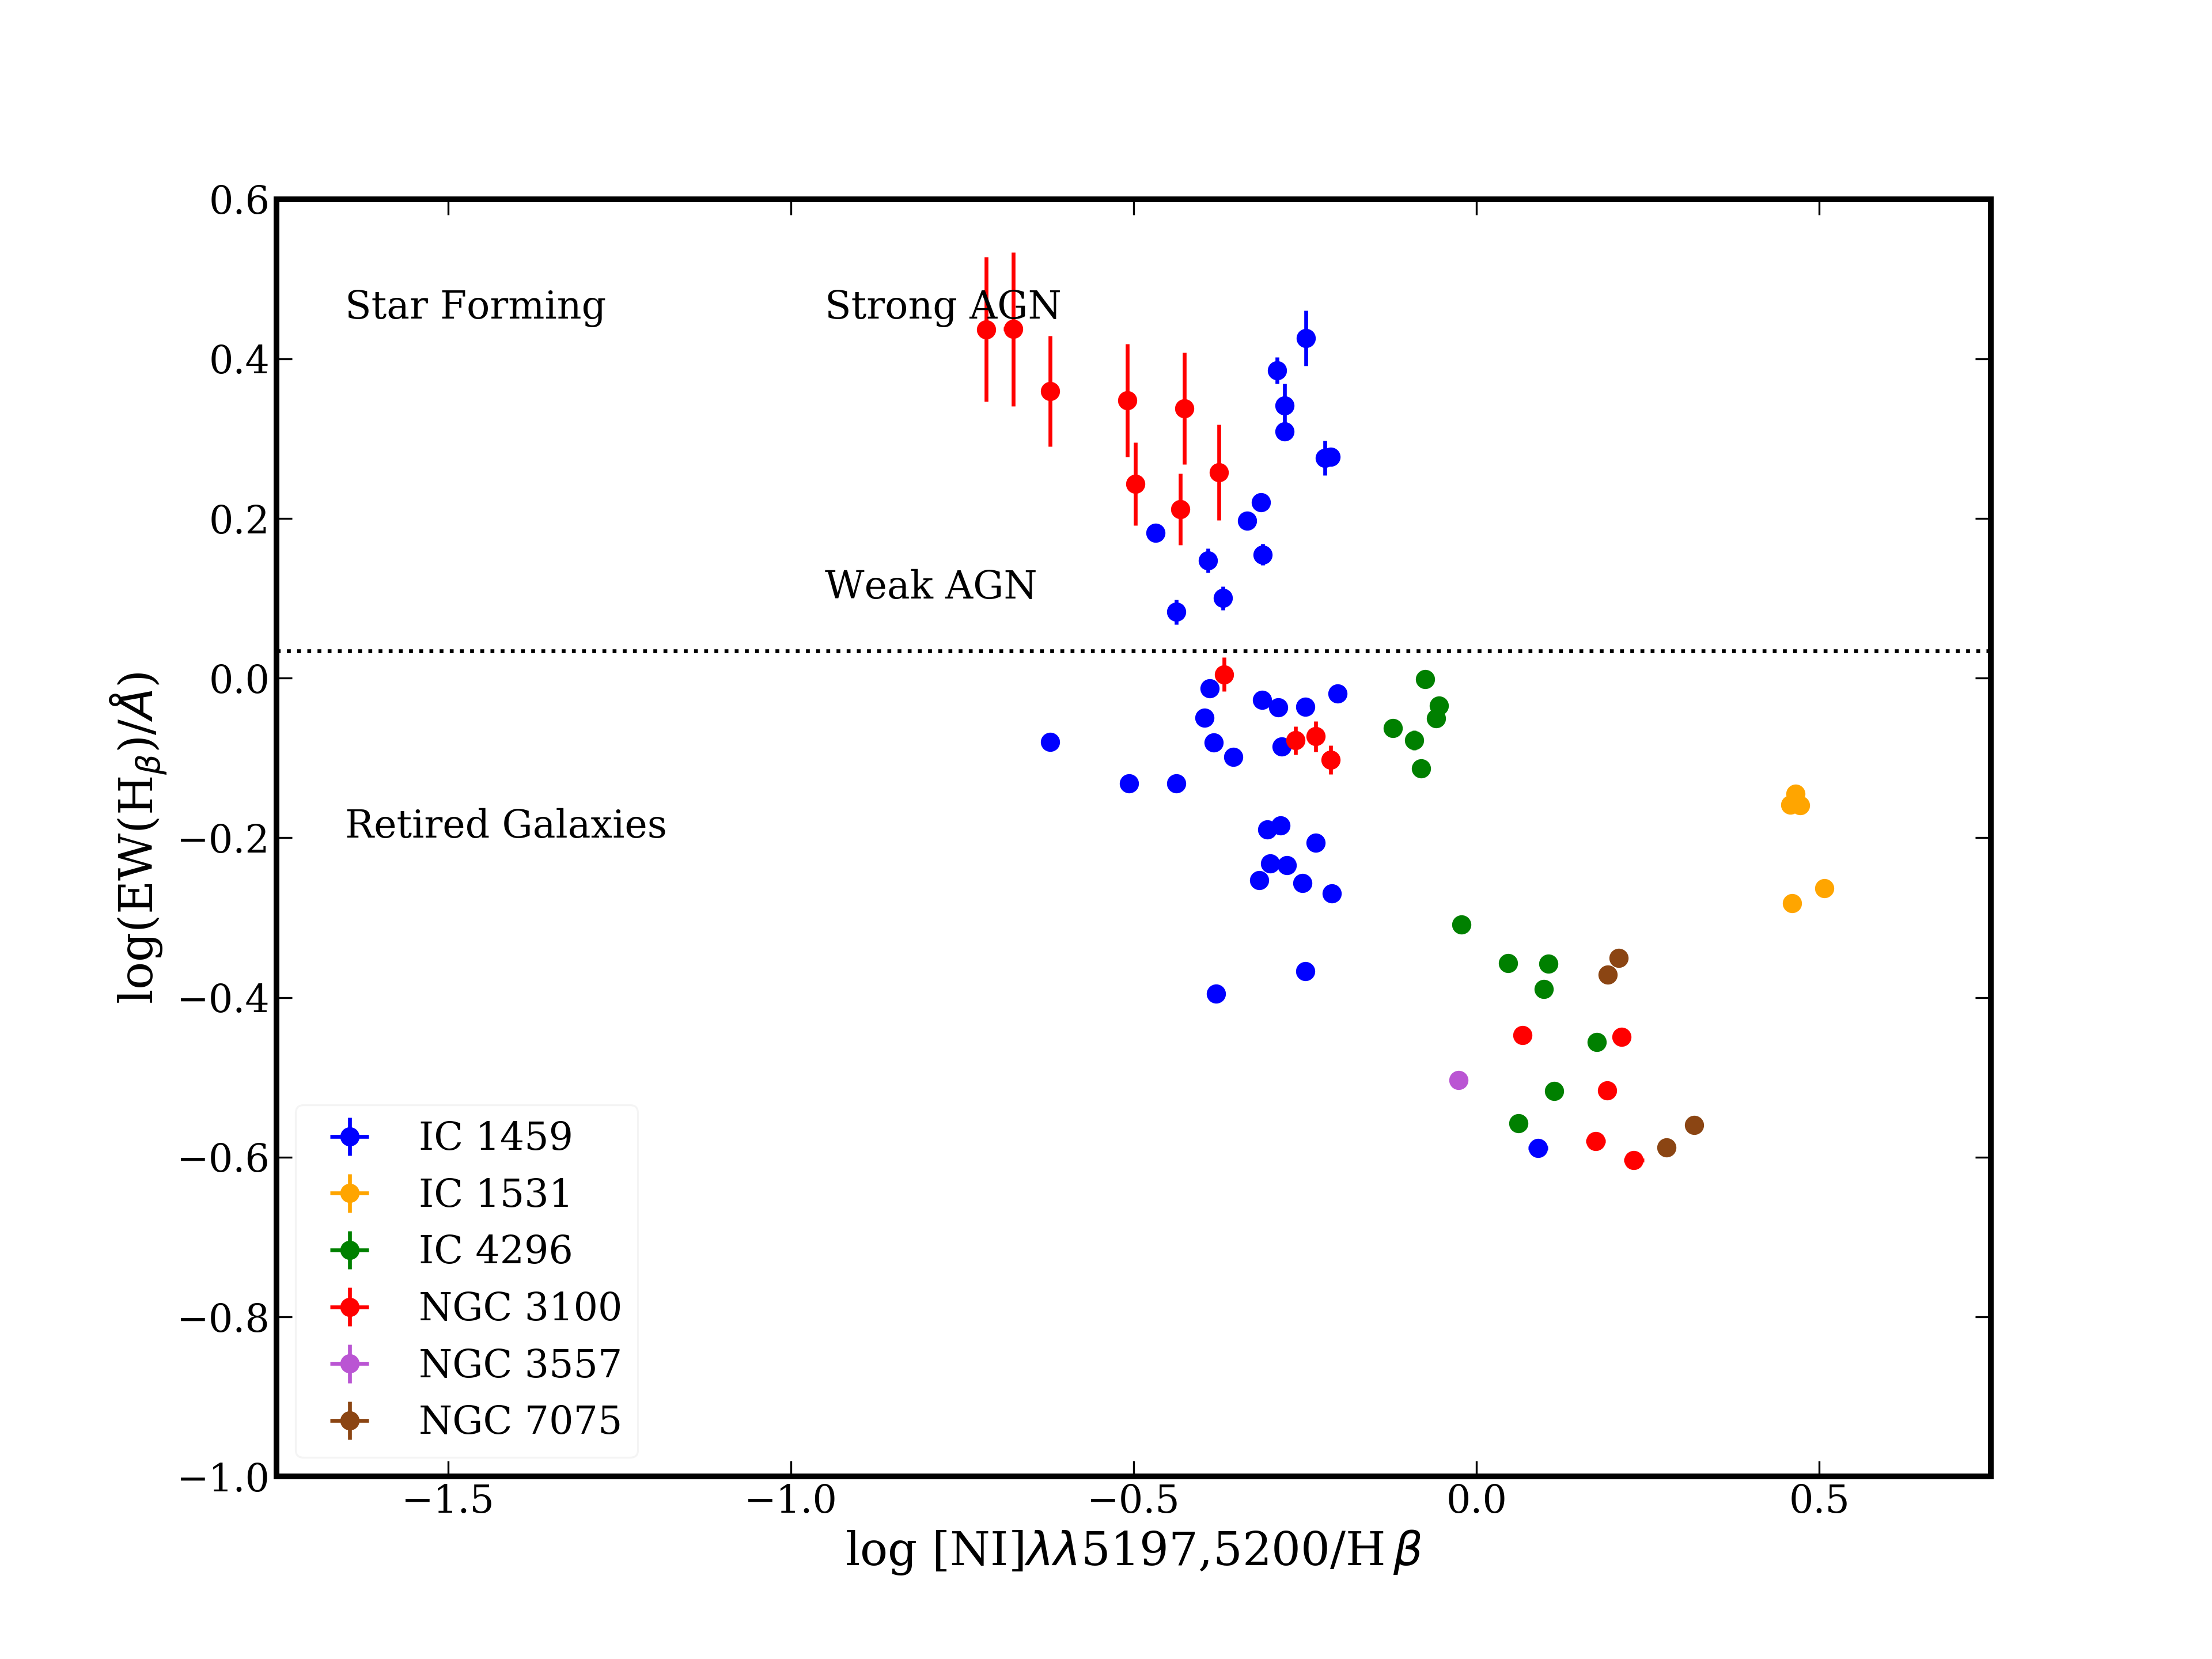
\includegraphics[width=0.8\textwidth]{chapter5/WHbN1.png}
			\caption[VIMOS WHbN1 plot]{VIMOS WHbN1 plot. All galaxies have decreasing H\,$\beta$ emission with increasing distance from the centre of the galaxy.}
			\label{fig:WHaN2}
		\end{figure}

% Comment on this


	\subsection{H\,$\beta$ profiles}
		\label{subsec:Hb}
		As discussed in Section \ref{sec:ETG} many galaxies classified as LINERs are in fact LIERs \citep[e.g.][]{Sarzi2005, Sarzi2010, Singh2013, Belfiore2016} i.e. the source of the ionising potential is not concentrated to the nuclear region of the galaxy. As we can see from Figs.\ref{fig:BPT} and \ref{fig:SAURON}, most bins are tightly grouped together on the BPT plots. In order to check if the ionizing radiation field is entirely due to the AGN throughout the entire host galaxy we plot the H\,$\alpha$ and H\,$\beta$ flux radial profiles for the MUSE and VIMOS data respectively. A point source, such as an AGN, will result in the profile having an $r^{-2}$ shape, where $r$ is the distance of the bin from the centre of the galaxy. A shallower profile points to a dispersed source, presumably non-circumnuclear stellar processes such as formation or radiation from post-asymptotic giant branch (pAGB) stars (see Section \ref{subsubsec:JetFeedback}), as the cause of the ionizing field in the outer parts of the galaxy (i.e. LIER rather than LINER). The profiles for our observations are shown in Figs.\,\ref{fig:Hb_profile_VIMOS} and \ref{fig:Ha_profile_MUSE}. All galaxies with spatially extended Balmer emission lines in our Southern sample show a central point source as the dominant source to the ionizing field. The plots with large scatter (NGC 612 and NGC 3100) suggest that stellar processes (likely to be radiation from pAGB stars considering these are ETGs and therefore are likely have very low star-formation rates) are also have an impact.

		\begin{figure}
			\centering
			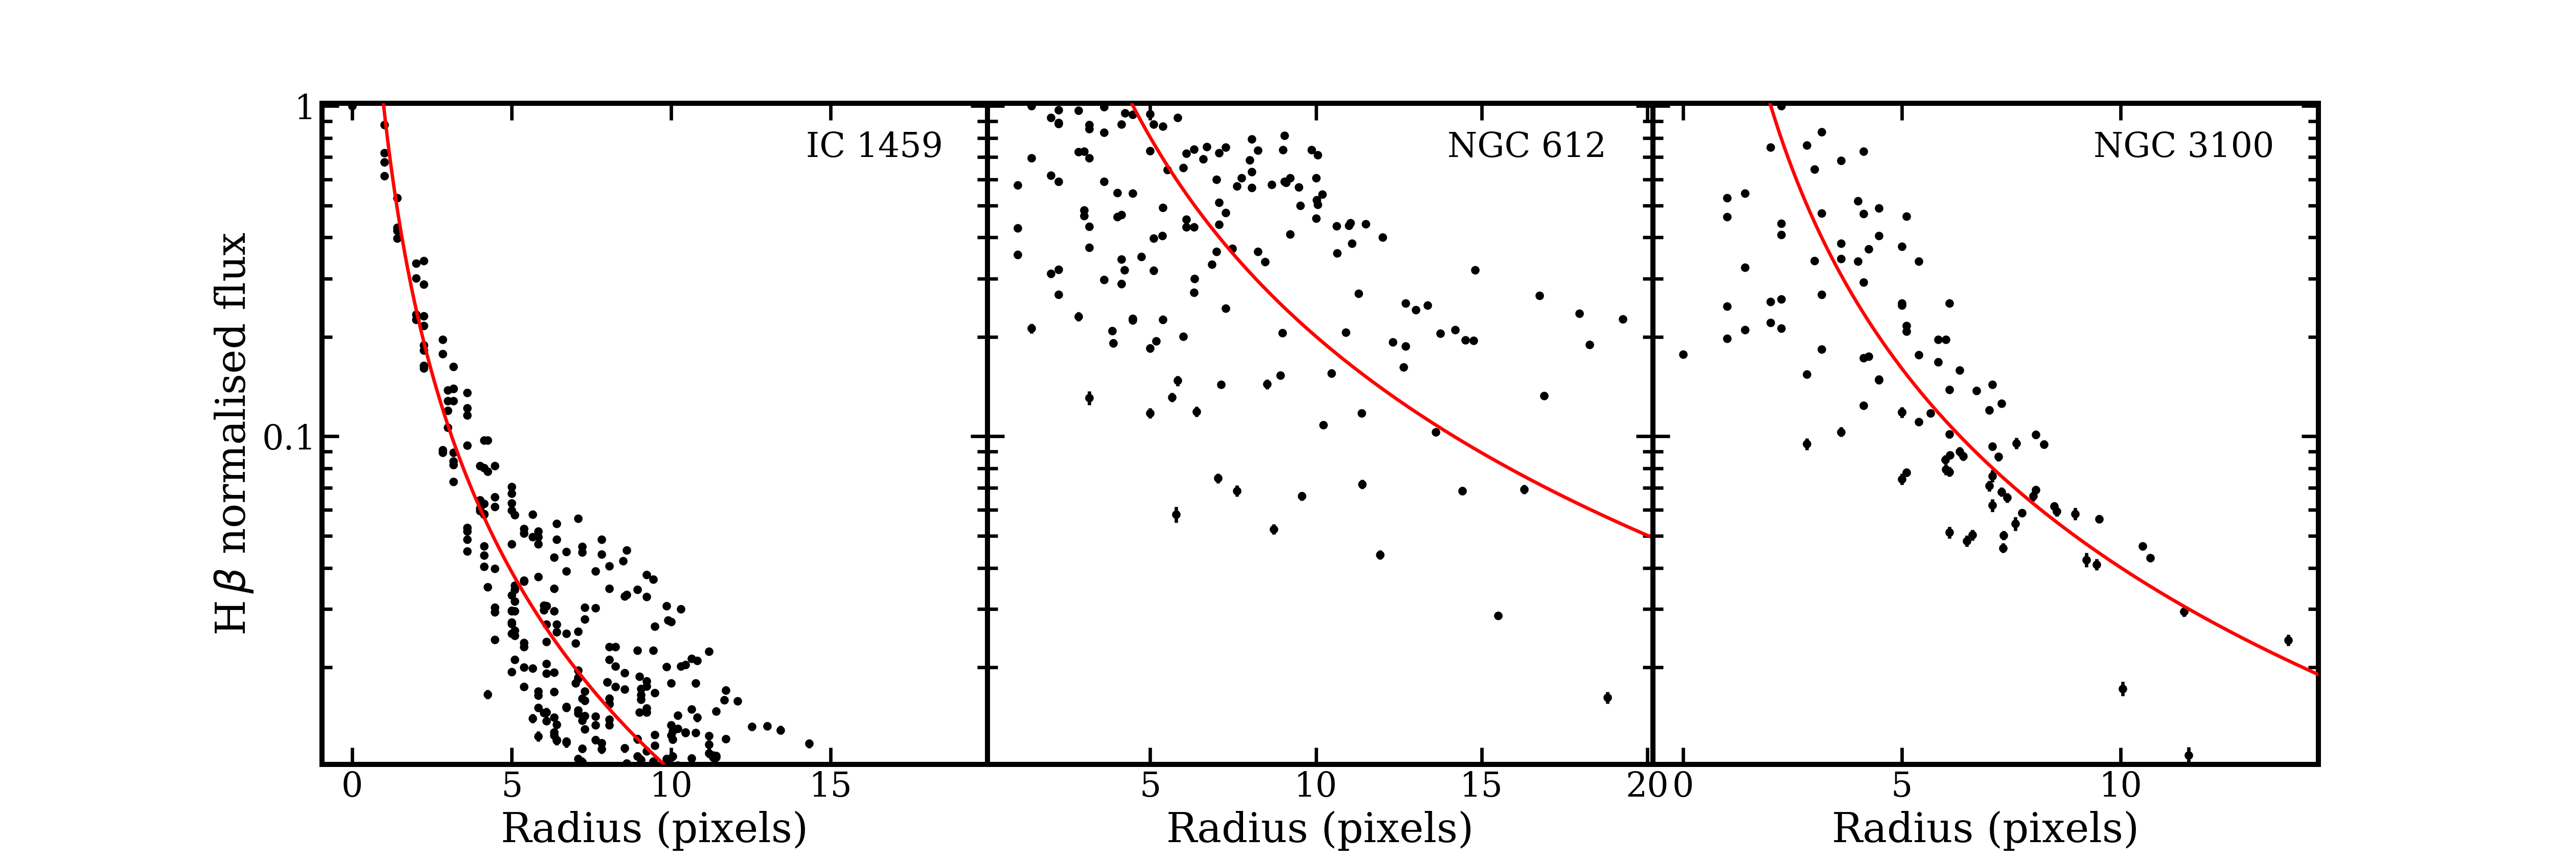
\includegraphics[width=\textwidth]{chapter5/vimos/Hbeta_profile.png}
			\caption[VIMOS H\,$\beta$ radial profiles]{H\,$\beta$ radial profiles derived from the VIMOS datacubes. Solid black line shows $H\,\beta \propto r^{-2}$.} 
			\label{fig:Hb_profile_VIMOS}
		\end{figure}

		\begin{figure}
			\centering
			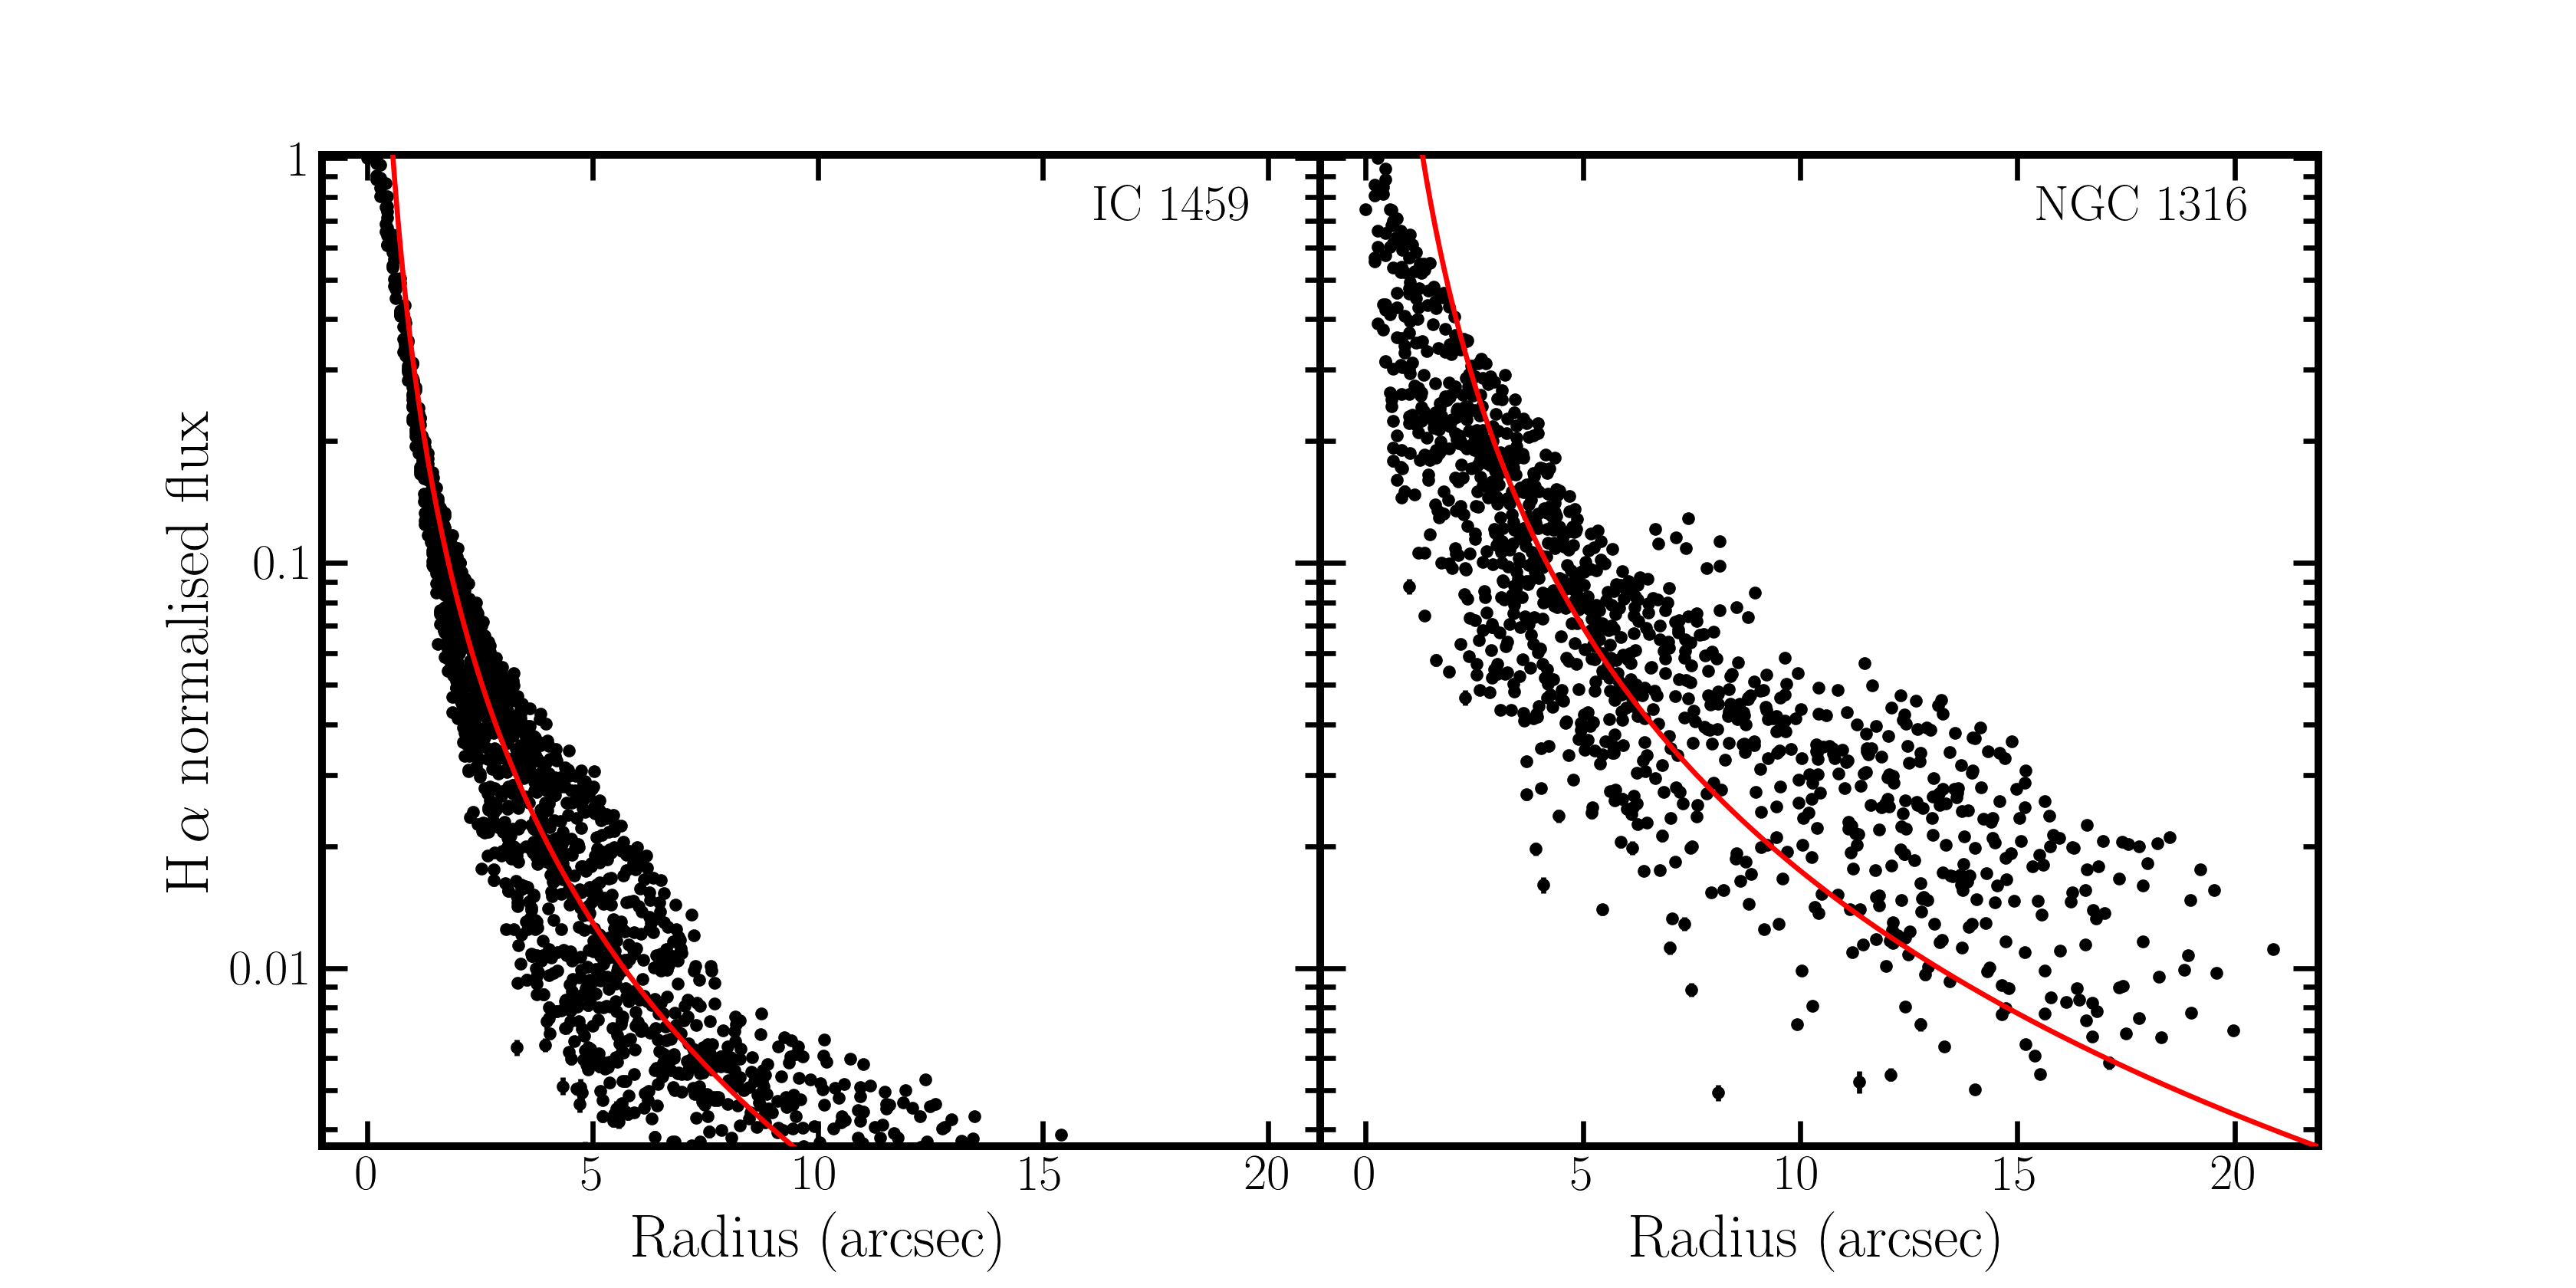
\includegraphics[width=0.66\textwidth]{chapter5/muse/Halpha_profile.png}
			\caption[MUSE H\,$\alpha$ radial profiles]{H\,$\alpha$ radial profiles derived from the MUSE datacubes. Solid black line shows $H\,\alpha \propto r^{-2}$.} 
			\label{fig:Ha_profile_MUSE}
		\end{figure}


	\subsection{MEx Diagnostic Plots}
		\label{subsec:MEx}
		The mass--excitation (MEx) plot of \citet{Juneau2011} is useful to classify galaxies with intermediate excitation levels ($0.5 < \mathrm{[\ion{O}{iii}]/H\,\beta} < 8.0$). It is particularly useful as it does not dependent on faint lines such as the [\ion{N}{I}] doublet. We use the calibrations by \citet{Nyland2016} including an attempt to separate LINERs powered by AGN from those powered by post-asymptotic giant branch (pABG) stars: the former have [\ion{O}{iii}] equivalent widths $>0.8$\,\AA. We use an aperture of 3$^\prime$ to plot the nuclear MEx for our Southern sample shown in Fig.\,\ref{fig:MEx}. 


		\begin{figure}
			\centering
			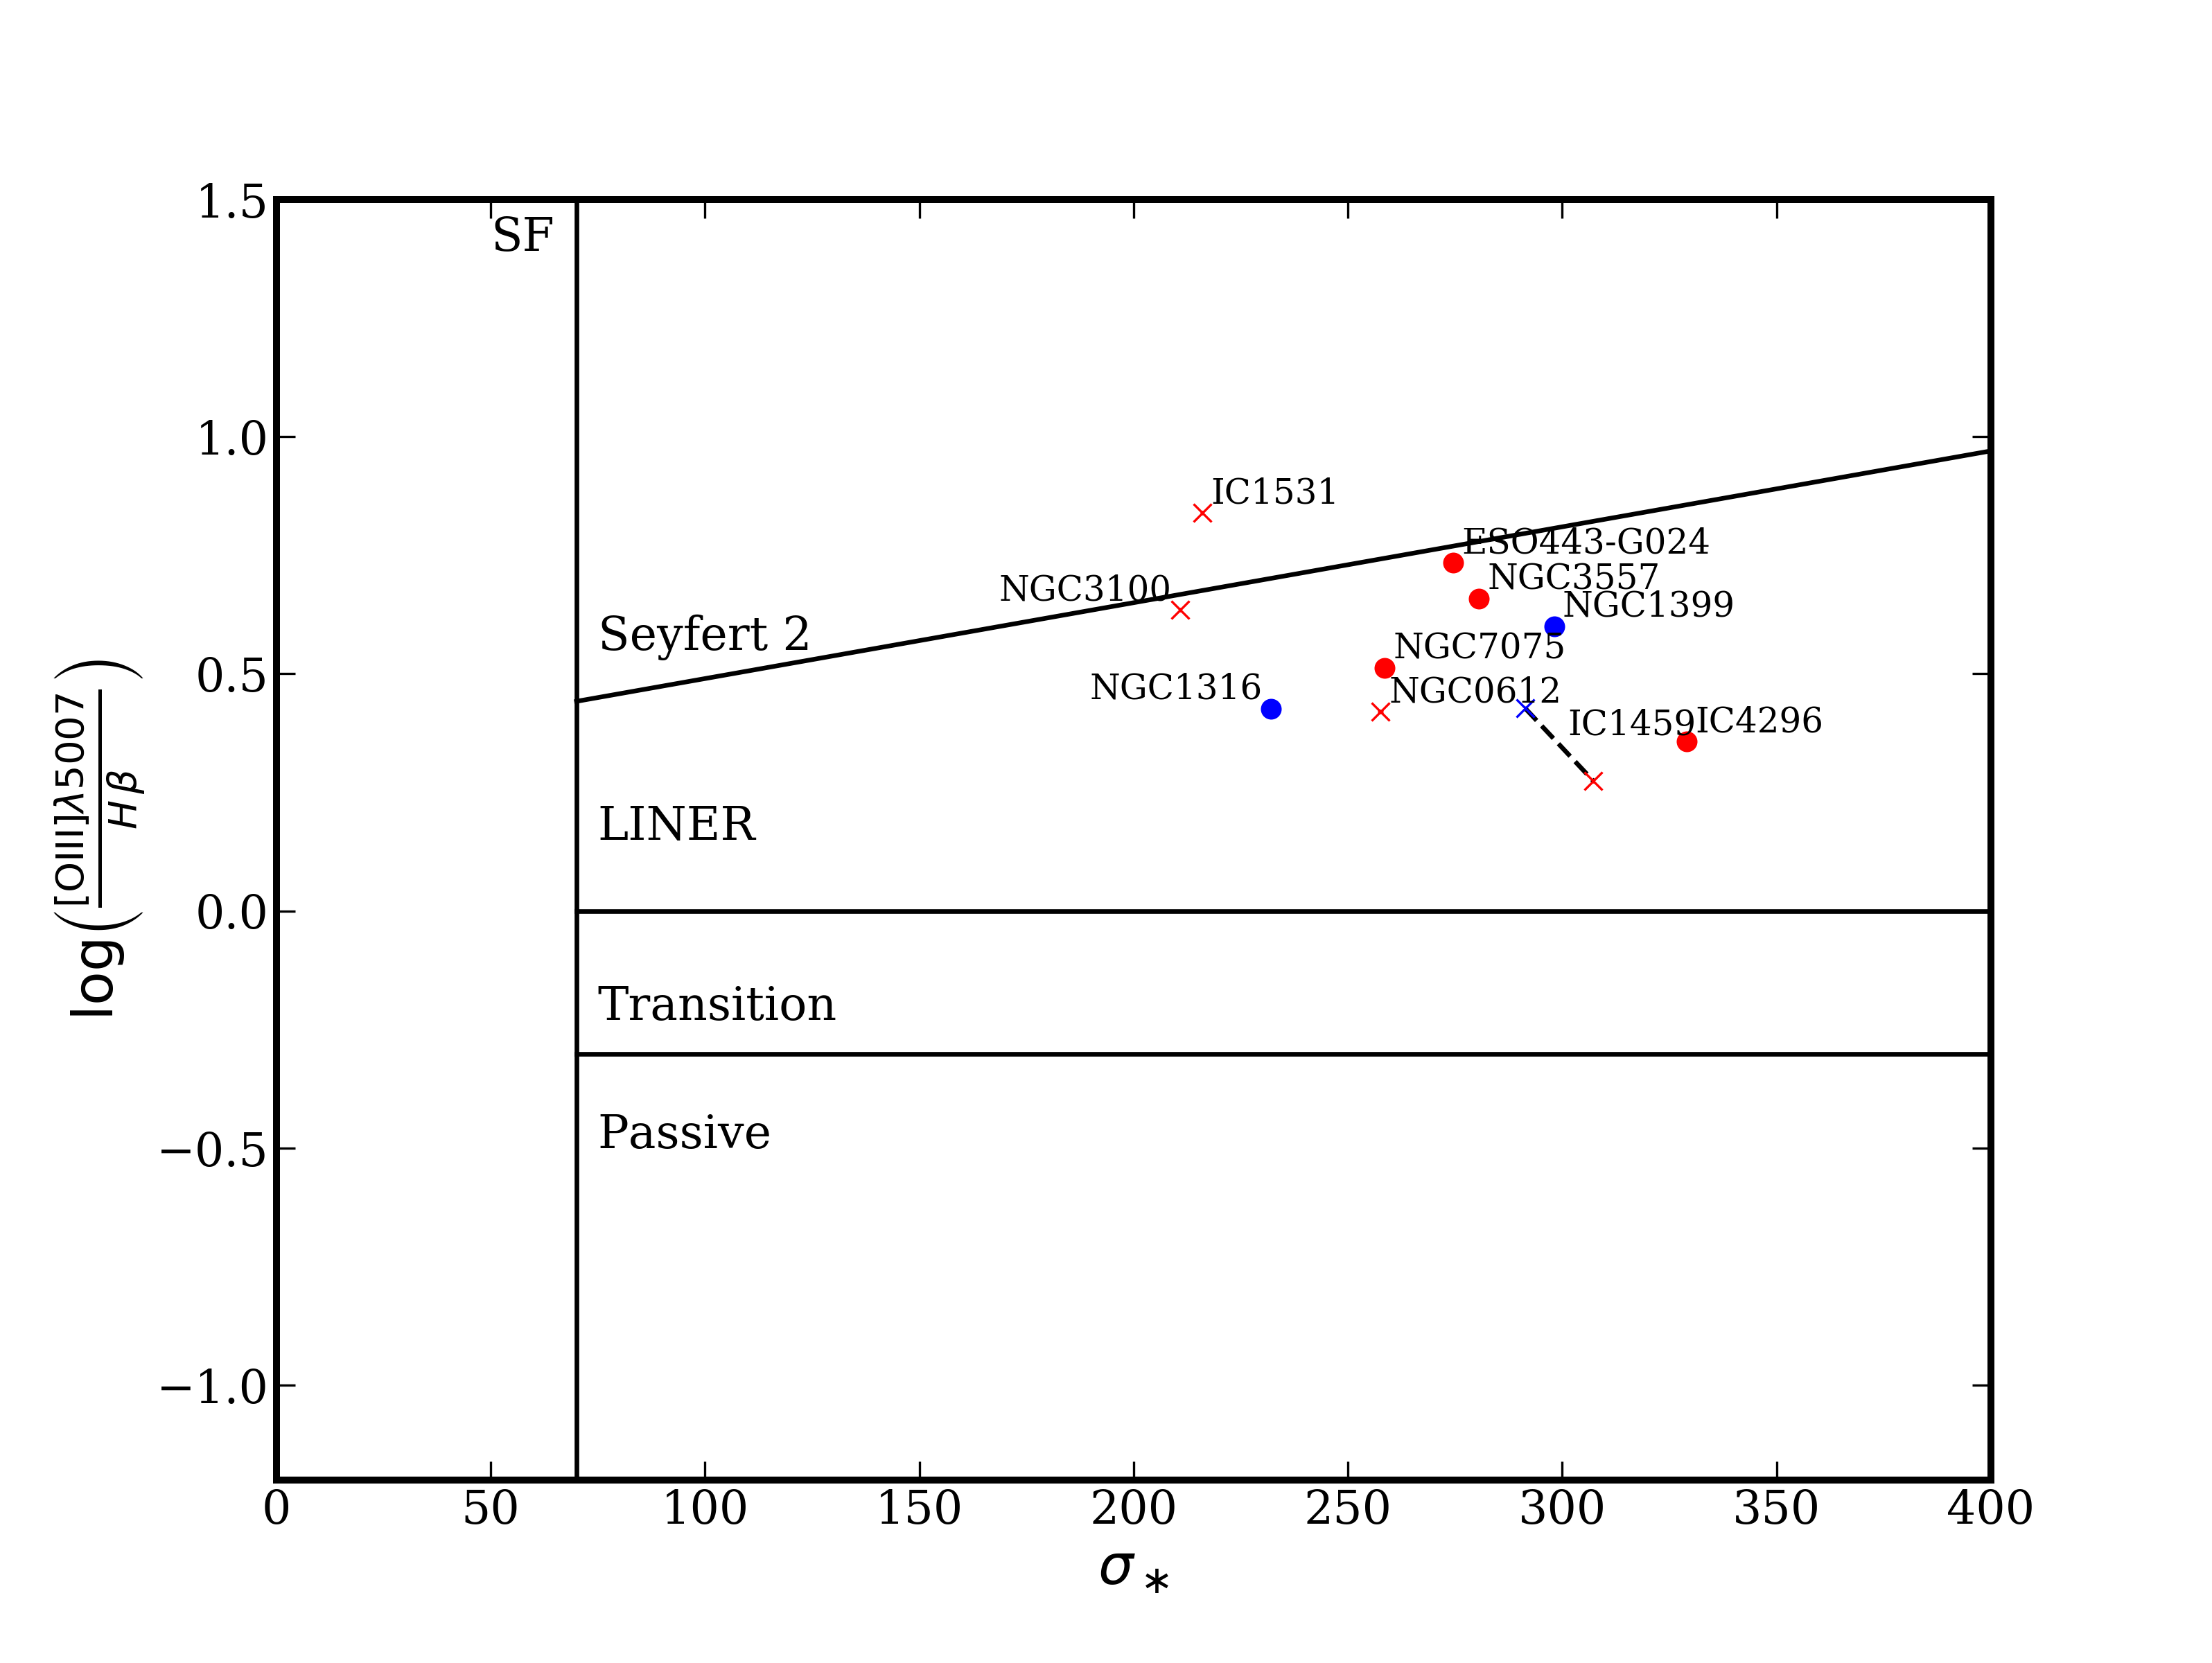
\includegraphics[width=0.8\textwidth]{chapter5/nuclear_MEx.png}
			\caption[Nuclear mass--excitation plot]{Nuclear MEx plot classifying the source of the ionizing radiation within the central 3$^\prime$. As in previous plots, points derived from VIMOS and MUSE datacubes are in red and blue, respectively. Crosses mark galaxies with [\ion{O}{iii}]$\lambda$5007 equivalent width of $> 0.8$\,\AA, while filled circles show galaxies with equivalent width of $\leqslant 0.8$\,\AA. The VIMOS and MUSE points of IC 1459 are linked with a black dashed line. Classification lines are from \citet{Nyland2016}.}
			\label{fig:MEx}
		\end{figure}



\section{Discussion}
	\label{sec:discuss}
% Check this paragraph. How did the results from whole_image.py turn out?
	In this chapter we have firstly shown that galaxies within our Southern sample have low masses ($10^2$--$10^3\,\mathrm{M_\odot}$ of ionized gas. These are within the typical masses observed in ETGs, albeit at the lower end. Given that our sample contains some of the most massive galaxies, this means that we observe very low gas fractions. 

	The only slow rotator with detected, spatially-extended ionized gas, IC 1459, show kinematic evidence that the gas has an external origin, although we do suggest that the gas may have been re-accreted after it was ejected during the merger that resulted in the KDC. 

	Of the other 3 galaxies with detected, spatially-extended gas (NGC 612, NGC 1316 and NGC 3100), we find that one, NGC 3100, shows kinematic evidence of an external origin to the gas; another, NGC 612, is consistent with an internal origin; while NGC 1316 is not clear, though is definitely not a settled disc. This is in keeping with the findings of \citet{Davis2011a} who shows that ($36\pm5$)\% of fast rotators have misaligned ionized gas kinematics with respect to the stellar kinematics, while slow rotators have a flat distribution of misalignments. This indicates that slow rotators are dominated by external sources of gas, while fast rotators can have either. 

	All galaxies in our Southern Sample with detectable emission lines show LINER (or LIER) or Seyfert 2 characteristics. The two galaxies that are classified as Seyfert 2s (NGC 612 and NGC 3100) are very close to the boundary line between Seyfert 2 and LINER. We observe that both galaxies classified as Seyfert 2s are fast rotators. This is consistent with \citet{Nyland2016}, who shows that all ETGs in the Atlas$^\text{3D}$ sample, classified as Seyferts are fast rotators. 

	Overall we find that our Southern sample is consistent with representing radio-detected, jet-mode AGN, which are ordinary ETGs experiencing an active phase, presumably due to the central black hole accreting gas in some form. 
